%%%%%%%%%%%%%%%%%%%%%%%%%% author.tex %%%%%%%%%%%%%%%%%%%%%%%%%
%
% sample root file for your contribution to a "contributed book"
%
% "contributed book"
%
% Use this file as a template for your own input.
%
%%%%%%%%%%%%%%%%%%%%%%%% Springer-Verlag %%%%%%%%%%%%%%%%%%%%%%%%%%

\documentclass{svmult}

\usepackage{amsmath}
\usepackage{amsfonts}
%\usepackage{amssymb}
\usepackage{color}
\usepackage{url}
\usepackage{verbatim}
\usepackage[dvipdfm]{graphicx} % add

%\usepackage{makeidx}         % allows index generation
\usepackage{graphicx}        % standard LaTeX graphics tool
                             % when including figure files
%\makeindex             % used for the subject index
                       % please use the style sprmidx.sty with
                       % your makeindex program

%%%%%%%%%%%%%%%%%%%%%%%%%%%%%%%%%%%%%%%%%%%%%%%%%%%%%%%%%%%%%%%%%%%%%
%\newtheorem{theorem}{Theorem}[section]
%\newtheorem{conjecture}[theorem]{Conjecture}
%\newtheorem{corollary}[theorem]{Corollary}
%\newtheorem{proposition}[theorem]{Proposition}
%\newtheorem{lemma}[theorem]{Lemma}
%\newdef{definition}[theorem]{Definition}
%\newdef{remark}[theorem]{Remark}

% \def\F2{{\mathbb F}_2}
% \def\wt{{\rm wt}}
% \def\wo{{\rm wt}_o}
% \def\wf{{\rm wt}_f}
% \def\UL{{\rm ul}}
% \def\bx{{{\mathbf x}}}
% \def\by{{{\mathbf y}}}
% \def\bz{{{\mathbf z}}}
% \def\bw{{{\mathbf w}}}
% \def\bu{{{\mathbf u}}}
% \def\im{{\mathrm{Im}}}
% \def\ker{{\mathrm{Ker}}}
% \def\id{{\mathrm{Id}}}
% \def\tr{{\mathrm{tr}}}

\def\bbf2{\ifmmode \mathbb{F}_2 \else $\mathbb{F}_2$ \fi}
%\newcommand{\bbf2}{{\ifmmode \mathbb{F}_2 \else $\mathbb{F}_2$ \fi}}

%%%%%%%%%%%%%%%%%%%%%%%%%%%%%%%%%%%%%%%%%%%%%%%%%%%%%%%%%%%%%%%%%%%%%
\begin{document}
%\newcommand{\bbf2}{\ifmmode \mathbb{F}_2 \else $\mathbb{F}_2$ \fi}
%%%%%%%%%%%%%%%%%%%%%%%%%%%%%%%%%%%%%%%%%%%%%%%%%%%%%%%%%%%%%%%%%%%%%

%\title*{Ultra-Fast Low-Discrepancy Points}
%\titlerunning{Fast Points}
\title*{A uniform real random number generator obeying the IEEE 754
  format using an affine transition \thanks{This study is partially
    supported by JSPS/MEXT Grant-in-Aid for Scientific Research
    No.18654021, No. 16204002, and JSPS Core-to-Core Program
    No.18005.}}

\titlerunning{SIMD-oriented Fast Mersenne Twister}

% \author{
% Usain Bolt\inst{1}\and
% Michael Phelps\inst{2}
% }
\author{Mutsuo Saito\inst{1}\and
Makoto Matsumoto\inst{2}}
% Use \authorrunning{Short Title} for an abbreviated version...
%
% \institute{
% Departement of Superhumans \\
% Lightning Yellow High School\\
% Kingston, Jamaica\\
% \url{http://en.wikipedia.org/wiki/Usain_Bolt}
% \and
% Deep Blue Swimming Pool \\
% University of Baltimore, USA \\
% \url{http://en.wikipedia.org/wiki/Michael_Phelps}
% }
\institute{
Dept.\ of Math.\ Hiroshima University
\texttt{saito@math.sci.hiroshima-u.ac.jp}
\and 
Dept.\ of Math.\ Hiroshima University
\texttt{m-mat@math.sci.hiroshima-u.ac.jp}
}

\maketitle
%%%%%%%%%%%%%%%%%%%%%%%%%%%%%%%%%%%%%%%%%%%%%%%%%%%%%%%%%%%%%%%%%%%%%
            
\begin{abstract} 
  % We proposed a fast pseudorandom number generator SFMT
  % (SIMD-orientd Fast Mersenne Twister) in MCQMC 2006.

  Here we propose a pseudorandom number generator specialized to
  generate double precision floating point numbers in IEEE 754 format.

  The idea is simple: to generate pseudorandom 64-bit patterns with
  the most significant 12-bit is specified, so that they represent
  real numbers in the range [1,2) obeying the IEEE 754 format in
  memory, using an $\mathbb{F}_2$ affine transition.

  Here, the affine means $x \mapsto Ax+c$ where
  $x$ is a state vector, $A$ is an $\mathbb{F}_2$
  matrix, and $c$ is a constant vector. This constant
  is necessary to fix the most significant bits.
  By a slight modification of the classical linear case,
  one can obtain the (lower bound of) period and the dimension of
  equi-distribution of the generator.

  Using SIMD instruction set, we designed dSFMT (double precision floating
  point SFMT), which generates two floating point numbers at one recursion.
  The generation speed is almost same or faster than Mersenne Twister's
  single precision floating point number generation.
\end{abstract}
%%%%%%%%%%%%%%%%%%%%%%%%%%%%%%%%%%%%%%%%%%%%%%%%%%%%%%%%%%%%%%%%%%%%%

\section {Introduction}
\label{sec:intro}

Recently, the scale of simulations is getting larger, and faster
pseudorandom number generators (PRNGs) are required. The power of CPUs
for usual personal computers are now sufficiently strong for such
purposes, and the necessity of efficient PRNGs for CPUs on PCs is
increasing.

We proposed a fast pseudorandom number generator SIMD-orientd Fast
Mersenne Twister (SFMT) \cite{SFMT} in MCQMC 2006.  SFMT is a successor
of Mersenne Twister (MT) \cite{MT} and faster than the original and
has better equidistribution property.

SFMT is based on a Single Instruction Multiple Data (SIMD) \cite{SIMD}
feature of recent CPUs. The specialization in hardware made speed up
of SFMT. We also proposed another specialization, block generation
which returns large block of pseudorandom numbers by one call.  
Both of them have been widely known as a techeneque of speed up.
%This
%kind of interfaces are widely known as a techeneque of speed up.
%, but
%not used for speed comparison of pseudorandom number generators
%(PRNGs) as far as we know.
Generally saying, specialization is a possible choice to
make a faster PRNG.

We are interested in scientific simulatios, and most scientific
Monte-Carlo simulation requires great deal of floating point
pseudorandom numbers.  In this article, we describe about a PRNG
specialized in generating floating point numbers.

% In this article, we use an additional specialization in high-speed
% generation for PRNGs.  We propose a PRNG specialized in double
% precision floating point numbers with the IEEE 754 format.
% We get an effcient recursion formula, using larger memory space.
%%%%%%%%%%%%%%%%%%%%%%%%%%%%%%%%%%%%%%%%%%%%%%%%%%%%%%%%%%%%%%%%%%%%%
\subsection{Generating floating point numbers}
\label{sec:floating}

Usually, floating point pseudorandom numbers are obtained by
converting integer pseudorandom numbers, because recursion in floating
point numbers accumulates errors, which sometimes have diffrent values
in diffrent CPUs. Generating integernumber numbers (which is exact and
fast) and converting it by multiplying a constant is usual way,
however this multiplication has conversion from a integer to
a floating point number, and the convertion is slow.

An idea to fasten the conversion is using bit operations on integer
number to fit to IEEE 754 floating point format. For example in C
language, to convert 64-bit interger \texttt{x} to double precision floating
point number \texttt{y} is done by:
\begin{verbatim}
 x = (x >> 12) | 0x3FF0000000000000ULL;
 y = *((double *)&x);
\end{verbatim}, more appropriate way in C is to use union.

This method was known at latest in 1997, Anger Fog used this
method in his open source library \cite{Fog}, but has not been
used very widly. Others found this method indepedently around
the year.

Another idea is to convert the unsigned integer to the same bit-sized
signed integer, then (signed) floating point number. The reason why
this method is fast is that implicit conversion uses double sized
signed intergers.

Thinking about \bbf2 -linear generator like MT, its recursion is done
in \bbf2 vector space and its output vectors are considered as
integers.  In this article, we propose an \bbf2 generator whose output
vectors can be regarded as floating point numbers.

%%%%%%%%%%%%%%%%%%%%%%%%%%%%%%%%%%%%%%%%%%%%%%%%%%%%%%%%%%%%%%%%%%%%%
\subsection{IEEE double precision floating point format}
\label{sec:ieee}

IEEE Standard for Binary Floating-Point Arithmetic (ANSI/IEEE Std
754-1985) \cite{ieee} is the most widely-used standard for
floating-point numbers.

\begin{center}
  \begin{figure}
    \caption{double precision floating point number \label{fig:ieee}}
    \includegraphics[width=0.7\linewidth]{ieee.eps}
  \end{figure}

  \begin{tabular}{|l|c|c|c|} \hline
    & exponent & fraction & represented number \\ \hline
    zero & 0 & 0 & $\pm 0$ \\ \hline
    denormalized number & 0 & $\neq$ 0 & $\pm 0.xxxx \times 2^{-1022}$ \\ \hline
    $\infty$ & 2047 & 0 & $\pm\infty$ \\ \hline
    NaN & 2047 & $\neq$ 0 & Not a Number \\ \hline
    normalized number & 
    other & any & 
    $\pm 1.xxxxx \times 2^{e - 1023}$ \\ \hline
    % \[ s \times (1 + f \times 2^{-52}) \times 2^{e - 1023} \]
    % \[ \pm 1.xxxxx \times 2^{e - 1023} \]
  \end{tabular}

  $xxxx$ shows the bit pattern of fraction part.
\end{center}

if sign bit is 0 and exponent part (11 bit) is 0x3ff,
then the format represent a normalized number in the range [1, 2).

Because of the format of normalized number, We decided to design a
PRNG whose output is uniformly distributed in the range [1, 2).  A
normalize number has additional 1 bit and the exponent part is
adjusted so that the integer part only has this additional 1 bit.
Therefore this format has 53-bit precision though it has only 52-bit
fraction part. On the other hand, our generator has 52-bit precision
because the exponent part is fixed.
%%%%%%%%%%%%%%%%%%%%%%%%%%%%%%%%%%%%%%%%%%%%%%%%%%%%%%%%%%%%%%%%%%%%%
\section{Theoretical base}
\label{sec:base}

Our new generator is based on Linear Feedback Shift Register (LFSR)
like MT. Moreover it has additional memory called `lung'.  LFSR with
additional memory is call Pulmonary LFSR.

\subsection{Pulmonary LFSR}
\label{sec:pulmonary}

% \begin{definition}
%   \begin{itemize}
%   \item A bit $\{0,1\}$ is identified with $\bbf2$, the two element
%     field.
%   \item $b$-bit memories in computer are identified with horizontal vectors in
%     $\bbf2^{b}$. 
%   \item We consider an array of $N$ $b$-bit in computer memory as the
%     vector space $(\bbf2^{b})^N$.
%   \end{itemize}
% \end{definition}

We identify the set of bit \{0, 1\} with the two element field \bbf2 .
This means that every arithmetic operation is done modulo 2.  A
$\mathbf{b}$-bit register or memory is identified with a vertical
vector in $\bbf2^b$, and $+$ denotes the sum as vectors (i.e.,
bit-wize exclusive or). We consider an array of $N$ $b$-bit in
computer memory as the vector space $(\bbf2^{b})^N$.

% \begin{definition}
%   Linear Feedbacked Shift Register (LFSR) is defined by a recursion
%   formula of rank $N$:
%   \[  \mathbf{w}_i = g(\mathbf{w}_{i-N}, ..., \mathbf{w}_{i-1}),  \]
%   where $g$ is an $\bbf2$-linear map $(\bbf2^{b})^N \rightarrow \bbf2^b$
%   and $\mathbf{w}_i \in \bbf2^b$.
% \end{definition}

An LFSR method is to generate a sequence $\mathbf{w_0}$,$\mathbf{w_1}$,
$\mathbf{w_2},...$ of elements $\bbf2^b$ by a recursion
\[ \mathbf{w}_{i+N} = g(\mathbf{w}_{i}, ..., \mathbf{w}_{i + N-1}), \]
where $g$ is an $\bbf2$-linear map $(\bbf2^{b})^N \rightarrow
\bbf2^b$.  In the implementation, this recursion is computed by using
an array \texttt{W[0...N-1]} of $N$ word of $b$-bit size, by the
simultanous substitutions
\[
\texttt{W[0]} \leftarrow \texttt{W[1]},\ 
\texttt{W[1]} \leftarrow \texttt{W[2]},\  \ldots,
\texttt{W[N-2]} \leftarrow \texttt{W[N-1]},\  
\texttt{[N-1]} \leftarrow
g(\texttt{W[0]},\ldots,\texttt{W[N-1]}). 
\]
The first $N-1$ substitutions shift the content of 
the array, hence the name of LFSR. 
Note that in the implementation we may use 
an indexing technique to avoid
computing these substitutions, see \cite[P.28 Algorithm A]{knuth:bible}.
Before starting the generation, we need to 
set some values to the state array, 
which is called the initialization. 

Mersenne Twister (MT) \cite{MT}
is an example with
\[
g(\mathbf{w}_0,\ldots,\mathbf{w}_{N-1})=(\mathbf{w}_0|\mathbf{w}_1)A + 
\mathbf{w}_M,
\]
where $(\mathbf{w}_0|\mathbf{w}_1)$ denotes
the concatenation of 
the $32-r$ most significant bits (MSBs) of $\mathbf{w}_0$ and 
the $r$ least significant bits (LSBs) of $\mathbf{w}_1$,
%and $A$ is a $(32\times 32)$-matrix 
$A$ is a $(32\times 32)$-matrix 
for which the multiplication $\mathbf{w} A$ is computable 
by a few bit-operations, and $M$ is an integer
($1 < M < N$).
Its period is $2^{32N-r}-1$, chosen to be a Mersenne prime.
To obtain a better equidistribution property, 
MT transforms the sequence by
a suitably chosen $(32\times 32)$ matrix $T$,
namely, MT outputs
$\mathbf{x}_0 T , \mathbf{x}_1 T, \mathbf{x}_2 T, \ldots$
(called tempering).

LFSR has a problem about slow recovery from the status 
which have many zero bits and little one bits \cite[\S 7]{well}.
A Pulmonary LFSR method is to generate a sequence
$\mathbf{w_0}$,$\mathbf{w_1}$, $\mathbf{w_2},...$ of elements
$\bbf2^b$ by a recursion
\begin{eqnarray*}
  \mathbf{w}_i &=& g(\mathbf{w}_{i-N+1}, ..., \mathbf{w}_{i-1},
  \mathbf{u}_{i-1}), \\
  \mathbf{u}_i &=& h(\mathbf{w}_{i-N+1}, ..., \mathbf{w}_{i-1},
  \mathbf{u}_{i-1}).
\end{eqnarray*}
where $g$ and $h$ are $\bbf2$-linear maps $(\bbf2^{b})^N \rightarrow \bbf2^b$
and $\mathbf{w}_i, \mathbf{u}_i \in \bbf2^b$.
In the implementation, $\mathbf{u_i}$ is expected to be kept in a
register of CPU.
The idea of Pulmonary LFSR was appeared in the talk of Hiroshi Haramoto
in MCM 2005, and used in WELL PRNG \cite{well} in 2006.

% figure~\ref{fig:plfsr} shows LFSR and Pulmonary LFSR.
% \begin{center}
%   \begin{figure}
%     \caption{Standard LFSR and Pulmonary LFSR \label{fig:plfsr}}
%     \hspace*{\fill}
%     \includegraphics[width=0.45\textwidth]{LFSR.pdf}
%     \hspace{\fill}
%     \includegraphics[width=0.45\textwidth]{puLFSR.pdf}
%     \hspace{\fill}
%   \end{figure}
% \end{center}
%%%%%%%%%%%%%%%%%%%%%%%%%%%%%%%%%%%%%%%%%%%%%%%%%%%%%%%%%%%%%%%%%%%%%
\section{Design of dSFMT}
\label{sec:dsfmt}

The aim of this article is to design and to implement a fast floating
point pseudorandom number generator with sufficient quality suitable
for large scale scientific simulation. We decided to use 128-bit
operation optimizable in SIMD feature of modern CPUs because we 
succeeded in SFMT.

We call our new generator dSFMT, which stands for double precision
floating point SIMD-oriented Fast Mersenne Twister. dSFMT is
specialized in generating double precesion floating point number in
IEEE 754 format.  We released dSFMT based on this idea in 2007 from
our web page\cite{web:dsfmt}.

Here we propose an improved version of dSFMT, dSFMT ver. 2.

\subsection{The recursion of dSFMT}
\label{sec:recursion}

dSFMT ver. 2 is a pulmonary LFSR, whose recursion formulas are:
\begin{eqnarray*}
  h(\mathbf{w}_0, ..., \mathbf{w}_{N-2}, \mathbf{u}_0)
  &=& A\mathbf{w}_{0} + \mathbf{w}_{M} + B\mathbf{u}_{0}, \\
  g(\mathbf{w}_0, ..., \mathbf{w}_{N-2}, \mathbf{u}_0)
  &=& \mathbf{w}_{0} 
  + Ch(\mathbf{w}_0, ..., \mathbf{w}_{N-2}, \mathbf{u}_0),
\end{eqnarray*}
where $\mathbf{w}_0$, $\mathbf{w}_M$, $\mathbf{w}_{N-2}$, and $u$ are
b(= 128) bit element of computer memory, regarding horizontal vectors
in $\bbf2^{128}$, and $A$, $B$, $C$ are sparse $128 \times 128$
matrices over \bbf2 for which $\mathbf{w}A$, $\mathbf{w}B$,
$\mathbf{w}C$ can be computed by a few SIMD operations. These vectors
are kept in an N elements array of computer memory, where
$\mathbf{w}_0$, ..., $\mathbf{w}_{N-2}$ are 0th to (N-2)th element and
u is the last element.

\begin{itemize}
\item 
  $\mathbf{w} A := \mathbf{w} \stackrel{64}{<<} p_1$

  This notation means that $\mathbf{w}$ is regarded as two 
  64-bit memories, and $\mathbf{w} A$ is the result of the left-shift
  of $\mathbf{w}$ by $p_1$ bits. There is such a SIMD operation in 
  Pentium SSE2, and PowerPC AltiVec SIMD can emulate it.
  $p_1$ is a parameter $12 \le p_1 < 64$.

\item
  $\mathbf{u} B := \mathbf{u}\textrm{perm(4, 3, 2, 1)}$

  This notation means that $\mathbf{u}$ is regarded as four
  32-bit memories and $\mathbf{u}\textrm{perm(4, 3, 2, 1)}$ is
  the result of reverse the order of 32-bit block in 128-bit.
  The permutation can be done by one SIMD operation.

\item 
  $\mathbf{u} C := (\mathbf{u} \stackrel{64}{>>} 12) 
  + (\mathbf{u} \& p_2)$

  The notation $\mathbf{u} \stackrel{64}{>>} 12$ means that
  $\mathbf{u}$ is regarded as two 64-bit memories like $A$ and
  right-shifted 12 bit.  And the notation $\&$ means 128-bit
  bitwise logical `\textbf{AND}' with a 128-bit constant vector $p_2$.
  $p_2$ is a concatination of two 64-bit vectors and each of them has
  12 bits of 0s in their most significant bits.

\end{itemize}
Here is a peice of code to show the recursion written in C language.
\begin{verbatim}
    u[0] = (w0[0] << p1) ^ wm[0] ^ (u0[1] >> 32) ^ (u0[1] << 32);
    u[1] = (w0[1] << p1) ^ wm[1] ^ (u0[0] >> 32) ^ (u0[0] << 32);
    w[0] = w0[0] ^ (u[0] >> 12) ^ (u[0] & p2[0]);
    w[0] = w0[1] ^ (u[1] >> 12) ^ (u[1] & p2[1]);
\end{verbatim}
where every array is defined to have two unsigned 64-bit integers
and \texttt{w0} is for $w_0$, and so on.

Fig.~\ref{fig:dsfmt} shows the recursion.
\begin{figure}
\caption{Diagram of dSFMT \label{fig:dsfmt}}
\begin{center}
\includegraphics[width=\linewidth]{fig-dsfmt.eps}
\end{center}
\end{figure}

\subsection{Parameter Search}
\label{sec:search}

To assure the least period of PRNG, we used Mersenne Prime. \cite{MT}
Parameters $M$, $p_1$, $p_2$ are randomly selected to fit the
condition that $0 < M < N - 1$
\end{document}
%%%%%%%%%%%%%%%%%%%%%%%%%%%%%%%%%%%%%%%%%%%%%%%%%%%%%%%%%%%%%%%%%%%%%
By trial and error, 
we searched for a set of parameters of SFMT,
with the period being a multiple of $2^{19937}-1$
and having good equidistribution properties.
The degree of recursion $N$ is $\lceil 19937/128 \rceil=156$, 
and the linear transformations $A,B,C,D$ are as follows.
\begin{itemize}
\item 
$\mathbf{w} A := (\mathbf{w} \stackrel{128}{<<} 8) + \mathbf{w}.$

This notation means that $\mathbf{w}$ is regarded
as a single 128-bit integer, and 
$\mathbf{w} A$ is the result of the left-shift
of $\mathbf{w}$ by 8 bits. There is such a SIMD operation
in both Pentium SSE2 and PowerPC AltiVec SIMD instruction 
sets (SSE2 permits only a multiple of 8
as the amount of shifting). 
Note that the notation $+$ means the exclusive-or
in this article.

\item
$\mathbf{w} B := (\mathbf{w} \stackrel{32}{>>} 11) \& (\mbox{\tt BFFFFFF6 BFFAFFFF DDFECB7F DFFFFFEF}).$

This notation means that $\mathbf{w}$ is considered to be 
a quadruple of $32$-bit integers, and
each $32$-bit integer is shifted to the right by 11 bits,
(thus the eleven most significant bits are filled with 0s, 
for each 32-bit integer).
The C-like notation $\&$ means the bitwise AND
with a constant 128-bit integer,
denoted in the hexadecimal form.

In the search,
this constant is generated as follows. 
Each bit in the 128-bit integer is independently 
randomly chosen, with the probability to choose 1 being $7/8$.
This is because we prefer to have more 1's for a denser 
feedback.

\item 
$\mathbf{w} C := (\mathbf{w} \stackrel{128}{>>} 8).$

%The notation 
%$(\mathbf{w} \stackrel{128}{>>} 8)$ 
This is the right shift of 
an 128-bit integer
by 8 bits, similar to the first.

\item
$\mathbf{w} D := (\mathbf{w} \stackrel{32}{<<} 18).$

Similar to the second,
$\mathbf{w}$ is cut into four pieces of 32-bit integers,
and each of these is shifted by 18 bits to the left.
\end{itemize}
All these instructions are available in 
both Intel Pentium's SSE2 and PowerPC's AltiVec SIMD instruction sets.
Figure~\ref{fig:SFMT-B2} shows a concrete description
of SFMT19937 generator with period a multiple of $2^{19937}-1$.
\begin{figure}
\begin{center}
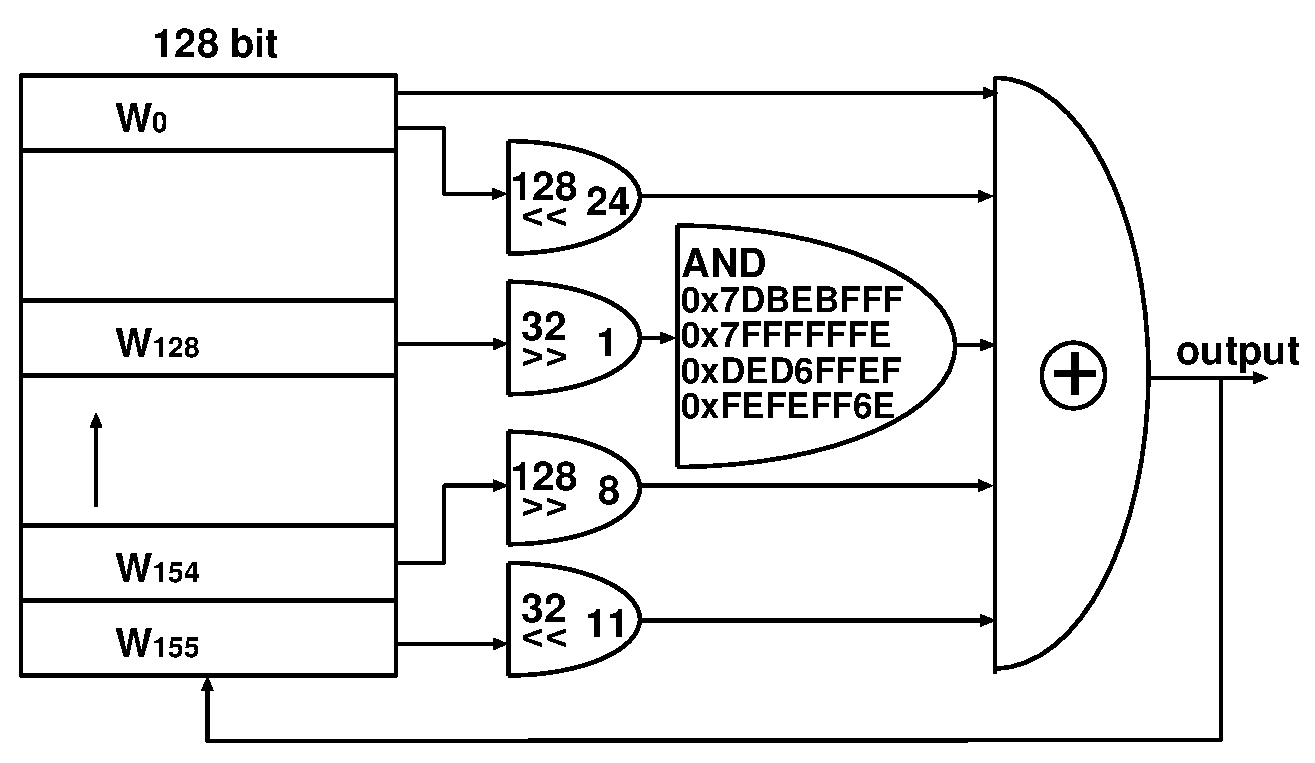
\includegraphics[width=0.5\linewidth]{sfmt-b2.eps}
\end{center}
\caption{A circuit-like description of SFMT19937.}
\label{fig:SFMT-B2}
\end{figure}
\subsection{Endianness}
Let $\mathbf{x}[0..3]$ be an array 
of 32-bit integers of size four.
There are two natural ways to convert the 
array to a 128-bit integer. One is to 
concatenate in the order of
$\mathbf{x}[3]\mathbf{x}[2]\mathbf{x}[1]\mathbf{x}[0]$, from MSBs to LSBs,
which is called the little-endian system, 
adopted in Pentium.
The converse is the big-endian system
adopted in PowerPC,
see \cite{wiki:endian}.

The descriptions in this article is based on the former.
To assure the portability for both endian systems, 
we implemented two codes: one is for little-endian 
system (SSE2 of Pentium) and the other is for
big-endian system (AltiVec of PowerPC), to 
assure the exactly same outputs 
as 32-bit integer generators.
In the latter code, the recursion (\ref{eq:rec-SFMT}) is considered as 
a recursion on quadruples of 32-bit integers, rather than
128-bit integers, so that the content of the state array 
coincides both for little and big endian systems,
as an array of 32-bit integers (not as 128-bit integers).
Thus, shift-operations on 128-bit integers in the little-endian
system is different from that in the big-endian system.
PowerPC supports arbitrary permutations of 
16 blocks of 8-bit integers in a 128-bit register,
which can emulate the shift in (\ref{eq:rec-SFMT}).

\subsection{Block-generation}\label{sec:block}
In the block-generation scheme, 
the user of the PRNG specifies an array
of $w$-bit integers of the length $L$, 
where $w=32$, 64 or 128 and $L$ is specified
by the user.
In the case of SFMT19937,
$wL$ should be a multiple of $128$
and no less than $N \times 128$,
since the array needs to accommodate the state space
(note that $N=156$).
By calling the block generation function 
with the pointer to this array, $w$, and $L$, 
the routine fills up the array with
pseudorandom integers, as follows. SFMT19937 keeps the state
space $S$ in an internal array of 128-bit integers of length 156.
We concatenate this state array with the user-specified array, 
using the indexing technique.
Then, the routine generates 128-bit integers in the user-specified 
array by recursion (\ref{eq:rec-SFMT}), as described
in Figure~\ref{fig:B1}, until it fills up the array.
The last 156 128-bit integers
are copied back to the internal array
of SFMT19937. 
This makes the generation much faster than sequential generation
(i.e., one generation per one call) as shown in Table~\ref{tab:speed}.
\begin{figure}
\begin{center}
%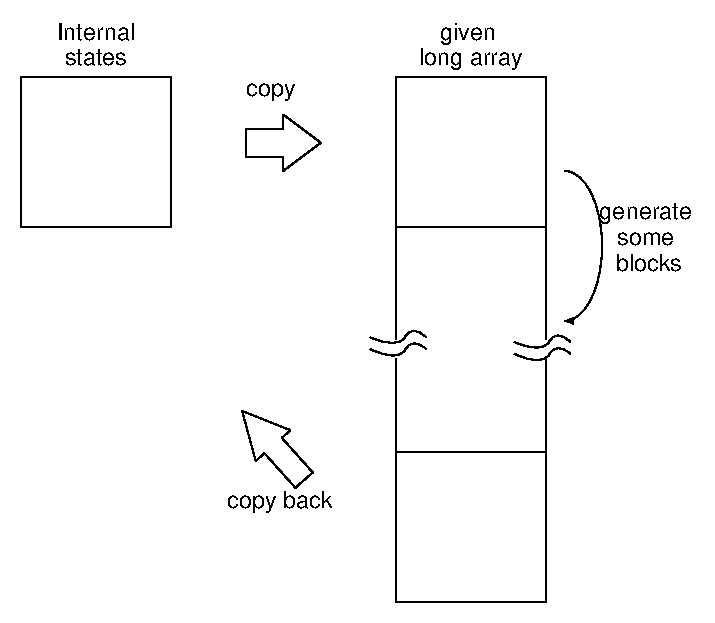
\includegraphics[width=0.7\linewidth,height=0.36\textheight,
\includegraphics[height=0.3\textheight,
keepaspectratio]{fill_array.eps}
\end{center}
\caption{Block-generation scheme}
\label{fig:B1}
\end{figure}

\section{How to select the recursion and parameters.}
We wrote a code to compute the period and
the dimensions of equidistribution (DE,
see \S\ref{sec:DE}). 
%Then, we search
Then, we searched
for a recursion with good DE admitting a fast implementation.  

\subsection{Computation of the Period}\label{sec:period}
%\subsection{Reducible transition function}
%LFSR by the recursion (\ref{eq:recursion})
An LFSR that obeys the recursion (\ref{eq:recursion})
may be considered as an automaton, 
with the state space $S=(\bbf2^{w})^{N}$
and the state transition function 
$f: S \to S$ given by
$(\mathbf{w}_0,\ldots,\mathbf{w}_{N-1})
\mapsto (\mathbf{w}_1,\ldots,\mathbf{w}_{N-1}, g(\mathbf{w}_0,\ldots,\mathbf{w}_{N-1}))$.  
As a $w$-bit integer generator, the output function is 
$o: S \to \bbf2^{w},\  (\mathbf{w}_0,\ldots,\mathbf{w}_{N-1}) \mapsto \mathbf{w}_0$.

Let $\chi_f$ be the characteristic polynomial of $f:S \to S$.
If $\chi_f$ is primitive, then the 
period of the state transition takes the maximal value
$2^{\dim(S)}-1$ \cite[\S3.2.2]{knuth:bible}. 
However, to check the primitivity, we need
the integer factorization of this number, which is often
hard for $\dim(S)=nw>10000$. 
On the other hand, the primarity test is much easier than 
the factorization, so many huge primes of the form 
$2^p-1$ have been found. 
Such a prime is called a Mersenne prime, and $p$ is
called the Mersenne exponent, which itself is a prime.

%MT and WELL\cite{WELL} discard some fixed $r$-bits from the
MT and WELL\cite{WELL} discard $r$ specific bits from the
array $S$, so that $nw-r$ is a Mersenne exponent. 
Then, the primitivity of $\chi_f$ is easily checked
by the algorithm in \cite[\S3.2.2]{knuth:bible},
avoiding the integer factorization.

SFMT adopted
another method to avoid the integer factorization,
the reducible transition method (RTM), 
which uses a reducible characteristic polynomial
with a large primitive factor.
This idea appeared in \cite{FUSHIMI90}
\cite{BRENT}\cite{BRENT-PRIM}, and 
applications in the present context are 
discussed in detail in another article \cite{PMT}, 
therefore we only briefly recall it. 

Let $p$ be the Mersenne exponent, and $N:=\lceil p/w \rceil$.
Then, we randomly choose parameters for the recursion of LFSR
(\ref{eq:recursion}).
By applying the Berlekamp-Massey Algorithm to 
the output sequence, we obtain 
$\chi_f(t)$.
%characteristiminimal polynomial of the transition function $f$.
%we compute the minimal polynomial of the (bit) sequence
%generated by the linear recursion. By taking the least
%common multiple for several initial values, we have the 
%minimal polynomial of the transition $f$. With high 
%probability its degree coincides with $\dim(S)$, and if 
%this occurs it is the characteristic polynomial $\chi_f$. 
(Note that a direct computation of $\det(tI-f)$ is time-consuming
 because $\dim(S)=19968$.)

By using a sieve, we remove all 
factors of small degree from $\chi_f$,
until we know that it has no irreducible factor of degree $p$,
or that it has a (possibly reducible) factor of degree $p$. 
In the latter case, the factor is 
passed to the primitivity test described 
in \cite[\S3.2.2]{knuth:bible}.

Suppose that we found a recursion with an irreducible factor of 
desired degree $p$ in $\chi_f(t)$. Then, 
we have a factorization
$$
\chi_f=\phi_p \phi_r,
$$
where $\phi_p$ is a primitive polynomial of degree $p$
and $\phi_r$ is a polynomial of degree $r = wN-p$. These are coprime, 
since we assume $p>r$.
%By putting $V_p:=\ker \phi_p(f)$ 
%and $V_r:=\ker \phi_r(f)$, 
Let $\ker(g)$ denote the kernel of a linear transformation $g$.
By putting $V_p:=\ker \left(\phi_p(f)\right)$ 
and $V_r:=\ker \left(\phi_r(f)\right)$,
we have a decomposition into $f$-invariant subspaces
$$
%S=V_p \oplus V_r,
S=V_p \oplus V_r \quad (\dim V_p=p, \ \dim V_r=r).
$$
Note that the characteristic polynomial of 
the restriction $f_p$ of $f$ to $V_p$ is $\phi_p(t)$, and
that of the restriction $f_r$ to $V_r$ is $\phi_r(t)$. 
For any state $s \in S$, we denote $s=s_p+s_r$ for the corresponding
decomposition with $s_p \in V_p$ and $s_r \in V_r$.
Then, the $k$-th state $f^k(s)$ is equal to
$f_p^k(s_p) + f_r^k(s_r)$. This implies that the automaton 
is equivalent to the sum of two automata $f_p:V_p \to V_p$ and
$f_r: V_r \to V_r$. To combine two linear automata by sum is 
well-studied as combined Tausworthe generators or combined LFSRs, 
see \cite{CLT} \cite{COMBTAUS} \cite{COMBLFSR}.
Their purpose is to obtain a good PRNG from several simple generators,
which is different from ours.

The period length of the state transition is the least common multiple
of that started from $s_p$ and that started from $s_r$. Hence, 
if $s_p \neq 0$, then the period is a nonzero multiple of $2^p-1$. 
We checked the following. 
\begin{proposition}
The period of SFMT19937 as a 128-bit integer generator is 
a nonzero multiple of $2^{19937}-1$, if the 32 MSBs of 
$\mathbf{w}_0$ are set to 
the value {\tt 6d736d6d} in hexadecimal form.
\end{proposition}
This value of $\mathbf{w}_0$ assures that $s_p\neq 0$,
see \cite{PMT} for a way to find such a value.

\begin{remark}
The number of non-zero terms in $\chi_f(t)$ is 
an index measuring the amount of bit-mixing. 
In the case of SFMT19937, the number of nonzero 
terms is 6711, which is much larger than 135 of MT, 
but smaller than 8585 of WELL19937c \cite{WELL}. 
\end{remark}

\subsection{Computation of the dimension of equidistribution}
\label{sec:DE}
We briefly recall the definition of dimension of 
equidistribution (cf. \cite{CLT}\cite{COMBTAUS}). 
\begin{definition}\label{def:DE}
A periodic sequence with period $P$
$$\chi:=\mathbf{x}_0, \mathbf{x}_1, \ldots, \mathbf{x}_{P-1}, \mathbf{x}_P=\mathbf{x}_0, \ldots$$
of $v$-bit integers is said to be {\em $k$-dimensionally equidistributed}
if any $kv$-bit pattern occurs equally often as a $k$-tuple
$$
(\mathbf{x}_i, \mathbf{x}_{i+1}, \ldots, \mathbf{x}_{i+k-1})
$$
for a period $i=0,\ldots, P-1$.
We allow an exception for 
the all-zero pattern, which may occur once less often.
(This last loosening of the condition is technically
necessary, because the zero state does not occur
in an $\bbf2$-linear generator). 
The largest value of such $k$ is called the dimension 
of equidistribution (DE).
\end{definition}

We want to generalize this definition slightly.
We define the $k$-window set of the periodic sequence $\chi$
as
$$
W_k(\chi):=
\{(\mathbf{x}_i, \mathbf{x}_{i+1}, \ldots, \mathbf{x}_{i+k-1}) | 
i =0,1,\ldots, P-1\},
$$
which is considered as a {\em multi-set}, namely, 
the multiplicity of each element is considered. 

For a positive integer $m$ and a multi-set $T$,
let us denote by $m \cdot T$ the multi-set 
where the multiplicity of each element in $T$ is
multiplied by $m$. Then, the above definition of
equidistribution is equivalent to 
$$
W_k(\chi)=(m\cdot \bbf2^{vk}) \setminus \{{\mathbf 0}\},
$$
where $m$ is the multiplicity of the occurrences,
and the operator $\setminus$ means that the multiplicity
of ${\mathbf 0}$ is subtracted by one. 

\begin{definition}
In the above setting, if there exist a positive integer $m$ 
and a multi-subset
$D \subset (m\cdot \bbf2^{vk})$
such that
$$
W_k(\chi)=(m\cdot \bbf2^{vk}) \setminus D,
$$
we say that $\chi$ is $k$-dimensionally equidistributed 
with defect ratio $\#(D)/\#(m \cdot \bbf2^{vk})$, 
where the cardinality is counted with multiplicity. 
\end{definition}
Thus, in Definition~\ref{def:DE}, the defect ratio up to $1/(P+1)$
is allowed to claim the dimension of equidistribution.
If $P=2^{19937}-1$, then $1/(P+1)=2^{-19937}$. 
In the following, the dimension of equidistribution 
allows the defect ratio up to $2^{-19937}$. 

For a $w$-bit integer sequence, its {\em dimension of 
equidistribution at $v$-bit accuracy} $k(v)$
is defined as the DE of the $v$-bit sequence, obtained by extracting
the $v$ MSBs from each of the $w$-bit integers.
If the defect ratio is $1/(P+1)$, 
then there is an upper bound 
$$
k(v) \leq \lfloor \log_2 (P+1) / v \rfloor.
$$
The gap between the realized $k(v)$ and the upper bound is
called the dimension defect at $v$ of the sequence,
and denoted by
$$
d(v):=\lfloor \log_2 (P+1) / v \rfloor -k(v).
$$
The summation of all the dimension defects at
$1 \leq v \leq 32$ is called the total dimension defect, 
denoted by $\Delta$.

There is a difficulty in computing $k(v)$ when 
a 128-bit integer generator is used as a 32-bit 
(or 64-bit) integer generator.
SFMT generates a sequence
$\mathbf{x}_0, \mathbf{x}_1, \mathbf{x}_2, \ldots$ of 128-bit integers. 
Then, they are converted to a sequence of 32-bit integers
$\mathbf{x}_0[0], \mathbf{x}_0[1], \mathbf{x}_0[2], \mathbf{x}_0[3], \mathbf{x}_1[0], \mathbf{x}_1[1],\ldots$,
where 
$\mathbf{x}[0]$ is the 32 LSBs of $\mathbf{x}$, 
$\mathbf{x}[1]$ is the 33rd--64th bits,
$\mathbf{x}[2]$ is the 65rd--96th bits,
and $\mathbf{x}[3]$ is the 32 MSBs. 
%(This is called the 
%little-endian system, see 
%\cite{wiki:endian}).
%for the notion of endianness, 
%and \S\ref{sec:portability} for
%an implementation in a big-endian system). 

Then, we need to modify the model automaton
as follows.
The state space is $S':=S \times \{0,1,2,3\}$,
the state transition function $f':S' \to S'$ is
$$
f'(s,i):=
\left\{
\begin{array}{cl}
(s, i+1) & (\mbox{ if $i<3$}), \\
(f(s), 0) & (\mbox{ if $i=3$}) \\
\end{array}
\right.
$$
and the output function is 
$$o': S' \to \bbf2^{32},\  ((\mathbf{w}_0,\ldots,\mathbf{w}_{N-1}),i) \mapsto \mathbf{w}_0[i].$$

We fix $1\leq v \leq w$, and let $o_k(s,i)$ be the $k$-tuple
of the $v$ MSBs of the consecutive $k$-outputs from 
the state $(s,i)$.
\begin{proposition}
Assume that $f$ is bijective.
Let $k'=k'(v)$ denote the maximum $k$ 
such that 
\begin{equation}\label{eq:chi-k-i}
%o_k(-,i): V_p \subset S \to \bbf2^{kv}, \quad s \mapsto o_k(s,i)
o_k(-,i): V_p \to \bbf2^{kv}, \quad s \mapsto o_k(s,i)
\end{equation}
are surjective for all $i=0,1,2,3$. 
%Take the initial state $s$ satisfying $s_p \neq 0$.
Take an initial state $s$ satisfying $s_p \neq 0$.
Then, the 32-bit output sequence is at least $k'(v)$-dimensionally
equidistributed with $v$-bit accuracy with defect ratio
$2^{-p}$.

Moreover, if $4 < k'(v)+1$, then  
for any initial state with $s=s_p \neq 0$
(hence $s_r=0$), the dimension of equidistribution
with defect ratio $2^{-p}$ is exactly $k'(v)$.
\end{proposition}
\begin{proof}
Take $s \in S$ with $s_p \neq 0$. Then, the 
orbit of $s$ by $f$ has the form of
$(V_p - \{0\}) \times U \subset V_p \times V_r$,
since $p>r$ and $2^p-1$ is a prime.
%Since the first component of the product has
%odd order, the orbit of $f'$ has the form of
%$(V_p - \{0\}) \times U' \times \{0,1,2,3\} \in S$.
The surjectivity of the linear mapping $o_{k'}(-,i)$
implies that the image of 
$$
o_{k'}(-,i): V_p \times U \to \bbf2^{kv}
$$
is $m\cdot \bbf2^{kv}$ as a multi-set for some $m$.
The defect comes from $0 \in V_p$, whose ratio
in $V_p$ is $2^{-p}$. Then the first statement follows,
since $W_{k'}(\chi)$ is the union of the images
$o_{k'}(-,i)((V_p-\{0\})\times U)$ for $i=0,1,2,3$.

For the latter half, we define
$L_i$ as the multiset of the image of 
$o_{k'+1}(-,i): V_p \to \bbf2^{(k'+1)v}$.
Because of $s_r=0$, we have $U=\{0\}$, and
the union of $(L_i-\{0\})$ $(i=0,1,2,3)$ as a multi-set is 
$W_{k'+1}(\chi)$. If the sequence is $(k'+1)$-dimensionally
equidistributed, then the multiplicity of
each element in $W_{k'+1}(\chi)$ is at most
$2^p\times 4/ 2^{(k'+1)v}$.

On the other hand, the multiplicity of 
an element in $L_i$ is equal to 
the cardinality of the kernel of $o_{k'+1}(-,i)$.
Let $d_i$ be its dimension. Then by the dimension theorem,
we have $d_i \geq p-(k'+1)v$, and the equality
holds if and only if $o_{k'+1}(-,i)$ is 
surjective.
Thus, if there is a nonzero element 
$x \in \cap_{i=0}^3{L_i}$, then its multiplicity
in $W_{k'+1}(\chi)$ is no less than 
$4 \times 2^{p-(k'+1)v}$, and since
one of $o_{k'+1}(-,i)$ is not surjective
by the definition of $k'$, its multiplicity
actually exceeds $4 \times 2^{p-(k'+1)v}$,
which implies that the sequence is not
$(k'+1)$-dimensionally equidistributed, and
the proposition follows. Since the codimension 
of $L_i$ is at most $v$, 
that of $\cap_{i=0}^3{L_i}$ is at most $4v$.
The assumed inequality on $k'$ implies the existence
of nonzero element in the intersection.
%
%Since the codimension of 
%each $L_i$ is at most $v$, the codimension of
%$\cap_{i=0}^3{L_i}$ is at most $4v$. The inequality
%in the assumption implies that there are at least 
%two nonzero vectors $x,y \in \cap_{i=0}^3{L_i}$.
%Now the inverse image of $x$ by $o_{k'+1}(-,i)$
%has the same cardinality with its kernel,
%hence $2^{p-\dim L_i}\geq 2^{p-(k'+1)v}$.
%
%If $W_{k'+1}(\chi)$ is $(k'+1)$-dimensionally
%equidistributed, then the inverse image of
%
\end{proof}

The dimension of equidistribution $k(v)$ depends on 
the choice of the initial state $s$. The above 
proposition implies that $k'(v)$ coincides 
with $k(v)$ for the worst choice of $s$ under the condition 
$s_p \neq 0$. Thus, we adopt the following definition
(analogously to $t_l$ in \cite{COMBTAUS}).

\begin{definition}\label{def:virtual}
Let $k$ be the maximum such that
(\ref{eq:chi-k-i}) is satisfied. We call this
the dimension of equidistribution
of $v$-bit accuracy, and denote it simply by $k(v)$.
We have an upper bound $k(v) \leq \lfloor p/v \rfloor$.

We define the dimension defect at $v$
%for SFMT19937 used as 32-bit integer generators
by
$$
d(v):=\lfloor p/v \rfloor - k(v) 
\mbox{ and } \Delta:=\sum_{v=1}^w d(v).
$$
\end{definition}
We may compute $k(v)$ by standard linear algebra.
We used a more efficient algorithm based on 
a weighted norm,
%{\em weighted lattice method} to compute $k'(v)$,
generalizing \cite{CLT}. This will be written 
somewhere else,
because of lack of space.
%rather complicated mathematics, we omit it here
%(we plan another article for this). 

%The algorithm gives a (rather tight) 
%lower bound $k'(v)$ of $k(v)$ for each $v$, 
%and $k'(v) \leq \lceil 19937/v \rceil$ holds
%for SFMT19937.
%Consequently, we redefine the dimension defect for SFMT19937 by
%$$
%d(v):=\lceil 19937/v \rceil - k'(v) 
%\mbox{ and } \Delta:=\sum_{v=1}^w d(v).
%$$
%The meaning of $k'(v)$ and a justification for this 
%definition will be explained in the planned article.

\section{Comparison of  speed}\label{sec:comp-speed}
We compared two algorithms: MT19937 and SFMT19937,
with implementations using and without using SIMD instructions.

We measured the speeds for four different CPUs:
Pentium M 1.4GHz, Pentium IV 3GHz, 
AMD Athlon 64 3800+, and PowerPC G4 1.33GHz.  
In returning the random values, we used two different methods.
One is sequential generation, where one 32-bit random 
integer is returned for one call. 
The other is block generation, where an array
of random integers is generated for one call 
(cf. \cite{knuth:bible}). 
For detail, see \S\ref{sec:block} below. 

We measured the consumed CPU time in second, 
for $10^8$ generations of 32-bit integers. More precisely,
in case of the block generation, we generate $10^5$
of 32-bit random integers by one call, and this is iterated
for $10^3$ times. 
For sequential generation, the same $10^8$
 32-bit integers are generated, one per call.
%To avoid the function call, the code uses 
%an inline declaration. 
We used the inline declaration
{\tt inline} to avoid the function call,
and unsigned 32-bit, 64-bit integer types 
{\tt uint32\_t}, {\tt uint64\_t} defined in 
INTERNATIONAL STANDARD ISO/IEC 9899 : 1999(E) 
Programming Language-C, Second Edition
(which we shall refer to as C99 in the rest of this article).
Implementations without SIMD are written in C99,
whereas those with SIMD use
some standard SIMD extension of C99 supported by 
the compilers icl (Intel C compiler) and gcc.

Table~\ref{tab:speed} summarises the speed comparisons.
 The first four lines list the CPU time
(in seconds) needed to generate $10^8$ 
32-bit integers, for a Pentium-M CPU with the Intel C/C++
compiler. The first line lists the seconds for the
block-generation scheme. The second line shows the 
ratio of CPU time to that of 
SFMT(SIMD). Thus, SFMT coded in SIMD is 2.10 times
faster than MT coded in SIMD, and 3.77 times faster
than MT without SIMD. The third line lists the seconds
for the sequential generation scheme. The fourth line
lists the ratio, with the basis taken
at SFMT(SIMD) block-generation (not sequential). 
Thus, the block-generation of SFMT(SIMD) is 2.00 times
faster than the sequential-generation of SFMT(SIMD).

Roughly speaking, in the block generation, 
SFMT(SIMD) is twice as fast as MT(SIMD),
and four times faster than MT without using SIMD.
Even in the sequential generation case,
SFMT(SIMD) is still considerably faster than MT(SIMD).

\begin{table}
\begin{center}
\begin{tabular}{|c|c||c|c|c|c|} \hline
CPU/compiler & return & MT & MT(SIMD) & SFMT & SFMT(SIMD)  \\ \hline \hline
Pentium-M & block & 1.122  & 0.627  & 0.689  & 0.298 \\ \cline{3-6}
1.4GHz & (ratio) & 3.77  & 2.10  & 2.31  & 1.00 \\ \cline{2-6}
Intel C/C++ & seq & 1.511  & 1.221  & 1.017  & 0.597 \\ \cline{3-6}
ver. 9.0 & (ratio) & 5.07  & 4.10  & 3.41  & 2.00 \\ \hline
Pentium IV & block & 0.633  & 0.391  & 0.412  & 0.217 \\ \cline{3-6}
3GHz & (ratio) & 2.92  & 1.80  & 1.90  & 1.00 \\ \cline{2-6}
Intel C/C++ & seq & 1.014  & 0.757  & 0.736  & 0.412 \\ \cline{3-6}
ver. 9.0 & (ratio) & 4.67  & 3.49  & 3.39  & 1.90 \\ \hline
Athlon 64 3800+ & block & 0.686  & 0.376  & 0.318  & 0.156 \\ \cline{3-6}
2.4GHz & (ratio) & 4.40  & 2.41  & 2.04  & 1.00 \\ \cline{2-6}
gcc & seq & 0.756  & 0.607  & 0.552  & 0.428 \\ \cline{3-6}
ver. 4.0.2 & (ratio) & 4.85  & 3.89  & 3.54  & 2.74 \\ \hline
PowerPC G4 & block & 1.089  & 0.490  & 0.914  & 0.235 \\ \cline{3-6}
1.33GHz & (ratio) & 4.63  & 2.09  & 3.89  & 1.00 \\ \cline{2-6}
gcc & seq & 1.794  & 1.358  & 1.645  & 0.701 \\ \cline{3-6}
ver. 4.0.0 & (ratio) & 7.63  & 5.78  & 7.00  & 2.98 \\ \hline
\end{tabular}
\end{center}
\caption{The CPU time (sec.) for $10^8$ generations of 32-bit integers,
for four different CPUs and two different return-value methods. 
The ratio to the SFMT coded in SIMD is listed, too.}\label{tab:speed}
\end{table}

\begin{table}
\begin{center}
\begin{tabular}{|c|c||c|c|c|c|c|c|}
\hline
CPU & return & mrg & rand48 & rand & random256g2 & well & xor3  \\ \hline \hline
Pentium M & block & 3.277  & 1.417  & 0.453  & 0.230  & 1.970  & 0.296 \\ 
\cline{2-8}
 & seq & 3.255  & 1.417  & 0.527  & 0.610  & 2.266  & 1.018 \\ \hline
Pentium IV & block & 2.295  & 1.285  & 0.416  & 0.121  & 0.919  & 0.328 \\ 
\cline{2-8}
 & seq & 2.395  & 1.304  & 0.413  & 0.392  & 1.033  & 0.702 \\ \hline
Athlon & block & 1.781  & 0.770  & 0.249  & 0.208  & 0.753  & 0.294 \\ 
\cline{2-8}
 & seq & 1.798  & 0.591  & 0.250  & 0.277  & 0.874  & 0.496 \\ \hline
PowerPC & block & 2.558  & 1.141  & 0.411  & 0.653  & 1.792  & 0.618 \\ 
\cline{2-8}
 & seq & 2.508  & 1.132  & 0.378  & 1.072  & 1.762  & 1.153 \\ \hline
\end{tabular}
\end{center}
\caption{The CPU time (sec.) for $10^8$ generations of 32-bit integers,
by six other PRNGs.}\label{tab:speed-other}
\end{table}
Table~\ref{tab:speed-other} lists the CPU time for generating
$10^8$ 32-bit integers, for four PRNGs from the GNU Scientific Library
and two recent generators. 
They are re-coded with inline specification. 
Generators examined were:
a multiple recursive generator {\tt mrg} \cite{MRG}, 
linear congruential generators {\tt rand48} and {\tt rand}, 
a lagged fibonacci generator {\tt random256g2},
a WELL generator {\tt well} (WELL19937c in \cite{WELL}),
and a XORSHIFT generator {\tt xor3} 
\cite{XORSHIFT} \cite{XORSHIFT-MAR}.
The table shows that SFMT(SIMD) is faster than
these PRNGs, except for the outdated
linear congruential generator {\tt rand},
the lagged-fibonacci
generator {\tt random256g2} 
(which is known to
 have poor randomness, cf. \cite{SUM}),
and {\tt xor3} with a Pentium-M.

\section{Dimension of equidistribution}
Table~\ref{tab:dd} lists the dimension defects $d(v)$
of SFMT19937 (as a 32-bit integer generator) 
and of MT19937, for $v=1,2,\ldots, 32$.
SFMT has smaller values of the defect $d(v)$
at 26 values of $v$. The converse holds for 6 values of
$v$, but the difference is small.
The total dimension defect $\Delta$ of SFMT19937
as a 32-bit integer generator is $4188$, 
which is smaller than the total dimension defect $6750$ of MT19937.

\begin{table}
\begin{center}
%\vskip -3mm
\begin{tabular}{|c|rr||c|rr||c|rr||c|rr|} \hline
$v$ & MT & SFMT & $v$ & MT & SFMT & $v$ & MT & SFMT & $v$ & MT & SFMT\\ \hline
$d(1)$ & 0 & 0 & $d(9)$ & 346 & 1 & $d(17)$ & 549 & 543 & $d(25)$ & 174 & 173 \\
$d(2)$ & 0 & *2 & $d(10)$ & 124 & 0 & $d(18)$ & 484 & 478 & $d(26)$ & 143 & 142
\\
$d(3)$ & 405 & 1 & $d(11)$ & 564 & 0 & $d(19)$ & 426 & 425 & $d(27)$ & 115 & 114
\\
$d(4)$ & 0 & *2 & $d(12)$ & 415 & 117 & $d(20)$ & 373 & 372 & $d(28)$ & 89 & 88
\\
$d(5)$ & 249 & 2 & $d(13)$ & 287 & 285 & $d(21)$ & 326 & 325 & $d(29)$ & 64 & 63
\\
$d(6)$ & 207 & 0 & $d(14)$ & 178 & 176 & $d(22)$ & 283 & 282 & $d(30)$ & 41 & 40
\\
$d(7)$ & 355 & 1 & $d(15)$ & 83 & *85 & $d(23)$ & 243 & 242 & $d(31)$ & 20 & 19 
\\
$d(8)$ & 0 & *1 & $d(16)$ & 0 & *2 & $d(24)$ & 207 & 206 & $d(32)$ & 0 & *1 \\
\hline
\end{tabular}
\end{center}
\caption{Dimension defects 
$d(v)$ of MT19937 and SFMT19937
as a 32-bit integer generator. 
The mark * means that MT has a smaller defect than SFMT
at that accuracy.
}\label{tab:dd}
\end{table}

%\begin{figure}
%\begin{center}
%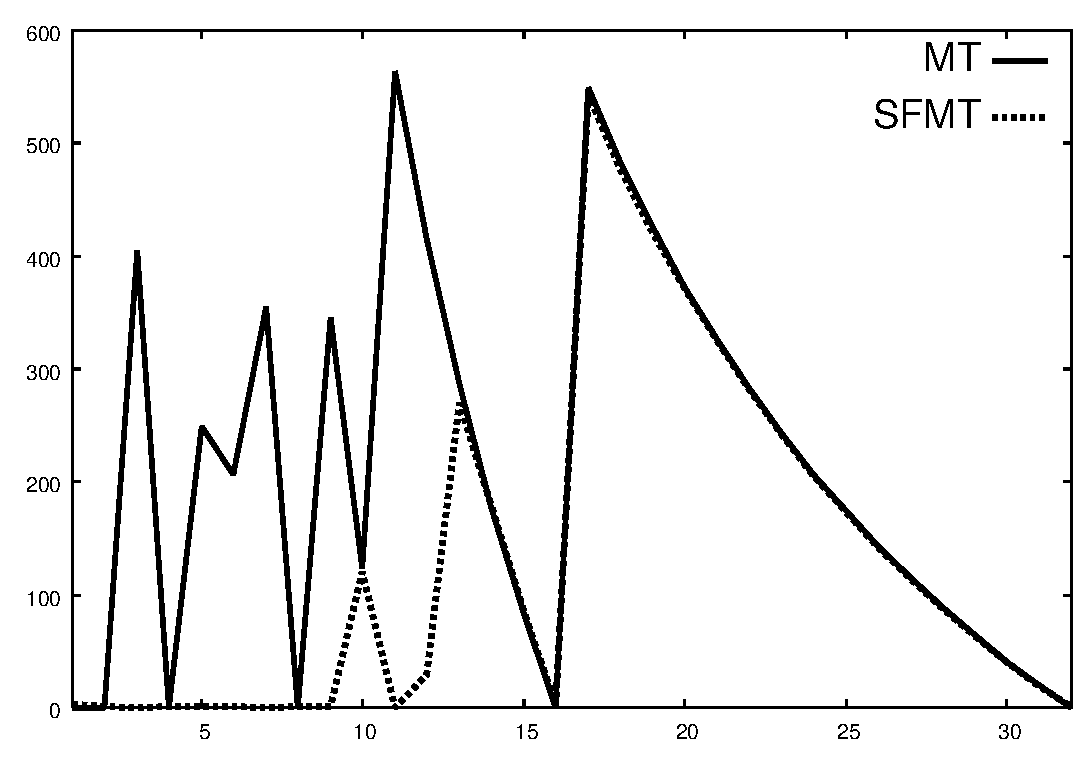
\includegraphics[width=0.8\linewidth,height=0.7\textheight,
%keepaspectratio]{delta.eps}
%\end{center}
%\caption{The dimension defects $d(v)$ of MT (real line) and 
%the dimension defects $d'(v)$ SFMT (dotted)
%for $v=1,2,\ldots, 32$.}
%\end{figure}

We also computed the dimension defects of SFMT19937 as a 64-bit
(128-bit) integer generator, and the total dimension 
defect $\Delta$ is 14089 (28676, respectively). In some applications, 
the distribution of LSBs is important. 
To check them, we inverted the order of the bits (i.e. the $i$-th
bit is exchanged with the $(w-i)$-th bit) in each integer, 
and computed the total dimension defect. It is
10328 (21337, 34577, respectively) as
a 32-bit (64-bit, 128-bit, respectively) integer generator.
Throughout the experiments, $d'(v)$ is very small for $v\leq 10$.
We consider that these values are satisfactorily small, since
they are comparable with MT
for which no statistical deviation
related to the dimension defect has been reported, 
as far as we know.

\section{Recovery from 0-excess states}
%LFSR with a sparse feedback function $g$ has
%the following phenomenon: 
For an LFSR with a sparse feedback function $g$,
we observe the following phenomenon: 
if the bits in the state space 
contain too many 0's and few 1's (called a 0-excess state), then
%this tendency continues for considerable generations,
this tendency continues for many steps,
since only a small part is changed in the state array
%at one generation, and the change is not well-reflected to 
%the next generation because of the sparseness.
at one step, and the change is not well-reflected to 
the next setp because of the sparseness.

We measure the recovery time from 0-excess states, 
by the method introduced in \cite{WELL}, as follows.
\begin{enumerate}
\item Choose an initial state with only one bit being 1.
\item Generate $k$ pseudorandom numbers, and discard them.
\item Compute the ratio of 1's among the 
next 32000 bits of outputs
(i.e., in the next 1000 pseudorandom 32-bit integers).
\item Let $\gamma_k$ be the average of the ratio over
all such initial states.
\end{enumerate}
We draw graphs of these ratio $\gamma_k$ $(1 \leq k \leq 20000)$
in Figure~\ref{fig:zero-recovery}
for the following generators: (1) WELL19937c, 
(2) PMT19937 \cite{PMT}, (3) SFMT19937, and (4) MT19937. 
%For (1), (2), (3) and (3), the chosen 
%initial states are those with only one bit being 1
%and all the rest 0. For (2*), the 32 MSBs in the first 128-bit
%integer in the state array is fixed to the value 
%{\tt 6d736d6d} in the hexadecimal form, and the initial states
%are those with only one bit being 1, except these 32 bits.
%Setting these 32 bits to this value assures that SFMT19937
%has the period being a nonzero multiple of $2^{19937}-1$,
%see \S\ref{sec:period}.
\begin{figure}
\begin{center}
\vskip -3mm
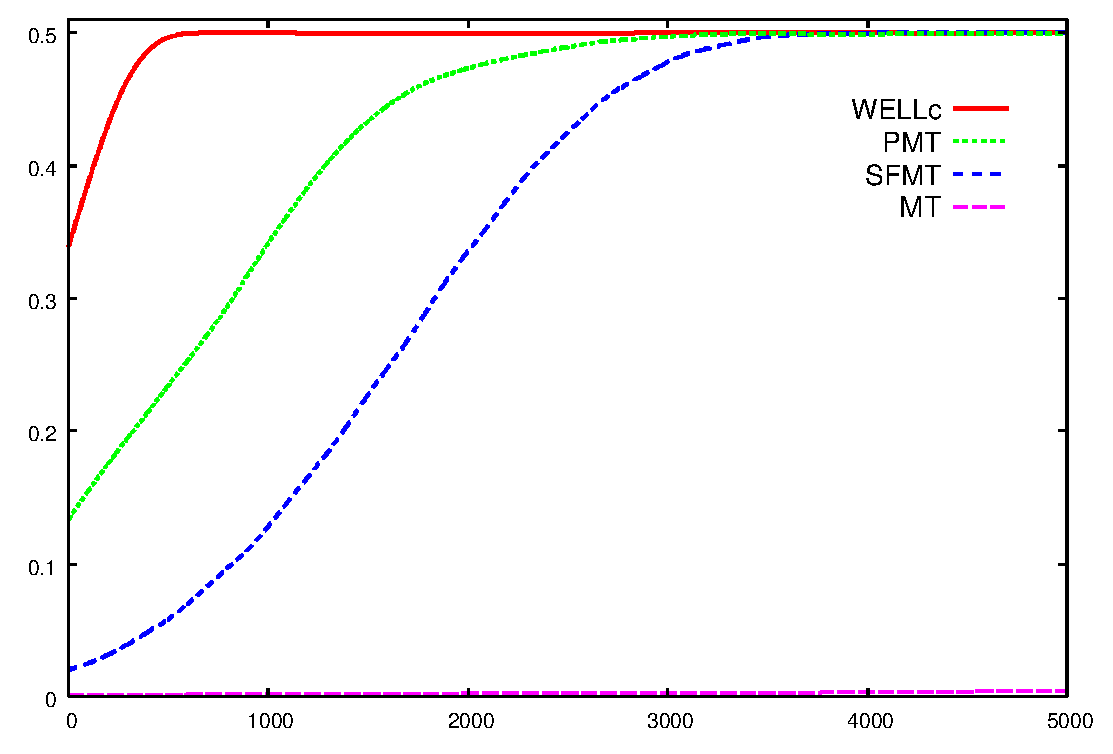
\includegraphics[width=0.7\linewidth]{sfmt-zero.eps}
\end{center}
\caption{$\gamma_k \ (k=0,\ldots,20000)$:
Starting from extreme 0-excess states,
discard the first $k$ outputs and then measure
the ratio $\gamma_k$ of 1's in the next 1000 outputs. 
In the order of the recovery speed: 
(1) WELL19937c, 
(2) PMT19937, (3) SFMT19937, and (3) MT19937.
}\label{fig:zero-recovery}
\end{figure}
Because of its dense feedback, WELL19937c shows
%the fastest recovery among the compared. 
the fastest recovery among the compared generators. 
SFMT is better than MT, since its recursion refers to 
%the previously-computed words (i.e., {\tt W[N-1]} and {\tt W[N-2]}) 
two most recently computed words ({\tt W[N-1]} and {\tt W[N-2]}) 
that acquire new 1s, while
MT refers only to the words generated long before 
({\tt W[M]} and {\tt W[0]}). PMT19937 shows faster recovery 
than SFMT19937, since PMT19937 has two feedback loops.
%(hence the name of Pulmonary Mersenne Twister).
The speed of recovery from 0-excess states 
is a trade-off 
with the speed of generation. 
Such 0-excess states will not happen practically, 
since the probability 
that 19937 random bits have less than $19937\times 0.4$ of 1's 
is about $5.7\times 10^{-177}$.
The only plausible case would be that
a poor initialization scheme gives a 0-excess initial state
(or gives two initial states whose Hamming distance is too small). 
In a typical simulation, the number of 
initializations is far smaller than the number of generations,
therefore we may spend more CPU time in the initialization
than the generation. Under the assumption that
a good initialization scheme is provided, the slower
recovery of SFMT compared to WELL would perhaps not be
a great issue.
% Once we avoid problematic initial states
%by a well-designed initialization, then the recovery 
%speed would not matter.%, in a practical sense. 
%We think the slower recovery of SFMT compared to WELL 
%would not be a great issue, under the assumption that
%a good initialization scheme is provided. 

\section{Concluding remarks}
%We proposed SFMT pseudorandom number generator, 
We proposed the SFMT pseudorandom number generator, 
which is a very fast generator with satisfactorily
high-dimensional equidistribution property. 

%\subsection{Trade-off between speed and quality}
It is difficult to measure the generation speed of a PRNG in a fair way,
since it depends heavily on the circumstances. 
The 
WELL \cite{WELL} generators have the best possible dimensions of 
equidistribution (i.e. $\Delta=0$)
for various periods ($2^{1024}-1$ to $2^{19937}-1$).
%If we use the function call to PRNG
If we use the function call to the PRNG
for each generation, then a large part of the CPU time
is consumed for handling the function call, and in the 
experiments in \cite{WELL} or \cite{XORSHIFT}, WELL 
is not much slower than MT. On the other hand, if we avoid
the function call, WELL is slower than MT for some CPUs, 
as seen in Table~\ref{tab:speed}. 

Since $\Delta=0$, WELL has a better quality than MT or SFMT
in a theoretical sense. 
However, one may argue whether this difference is 
observable or not. In the case of an $\bbf2$-linear generator,
the dimension of equidistribution $k(v)$ of $v$-bit accuracy
means that
there is no constant linear relation among the 
$kv$ bits, but there exists a linear relation among
the $(k+1)v$ bits, where $kv$ bits 
($(k+1)v$ bits) are taken from
all the consecutive $k$ integers 
($k+1$ integers, respectively)
by extracting the $v$ MSBs from each.
However, the existence of a linear relation does not necessarily
mean the existence of some observable bias.
According to \cite{TESTWEIGHT}, it requires $10^{28}$
samples to detect an $\bbf2$-linear relation with 
15 (or more) terms among 521 bits, by weight distribution test. 
If the number of 
bits is increased, 
the necessary sample size is increased rapidly. Thus, it seems
that $k(v)$ of SFMT19937 is sufficiently large, far beyond
the level of the observable bias. 
On the other hand, the speed of the generator is 
observable.
Thus, SFMT focuses more on the speed, for applications
that require fast generations. 
(Note: the referee pointed out that statistical
tests based on the rank of $\bbf2$-matrix is sensitive to 
the linear relations \cite{TESTU01}, 
so the above observation is not necessarily true.)

%\subsection{Trade-off between speed and portability}\label{sec:portability}
There is a trade-off between the speed and portability.
%We prepare (1) a standard C code of SFMT, which uses 
We prepared (1) a standard C code of SFMT, which uses 
functions specified in C99 only, (2) an optimized C code for
Intel Pentium SSE2, and 
(3) an optimized C code for PowerPC AltiVec. The optimized codes require
%icl (Intel C Compiler) or gcc compiler with suitable options.
the icl (Intel C Compiler) or gcc compiler with suitable options.
We had put and will keep the newest version of the codes 
in the homepage \cite{SFMT}.

\bibliographystyle{plain}
\bibliography{sfmt-kanren}
%%%%%%%%%%%%%%%%%%%%%%%%%%% author.tex %%%%%%%%%%%%%%%%%%%%%%%%%
%
% sample root file for your contribution to a "contributed book"
%
% "contributed book"
%
% Use this file as a template for your own input.
%
%%%%%%%%%%%%%%%%%%%%%%%% Springer-Verlag %%%%%%%%%%%%%%%%%%%%%%%%%%

\documentclass{svmult}

\usepackage{amsmath}
\usepackage{amsfonts}
%\usepackage{amssymb}
\usepackage{color}
\usepackage{url}
\usepackage{verbatim}
\usepackage[dvipdfm]{graphicx} % add

%\usepackage{makeidx}         % allows index generation
\usepackage{graphicx}        % standard LaTeX graphics tool
                             % when including figure files
%\makeindex             % used for the subject index
                       % please use the style sprmidx.sty with
                       % your makeindex program

%%%%%%%%%%%%%%%%%%%%%%%%%%%%%%%%%%%%%%%%%%%%%%%%%%%%%%%%%%%%%%%%%%%%%
%\newtheorem{theorem}{Theorem}[section]
%\newtheorem{conjecture}[theorem]{Conjecture}
%\newtheorem{corollary}[theorem]{Corollary}
%\newtheorem{proposition}[theorem]{Proposition}
%\newtheorem{lemma}[theorem]{Lemma}
%\newdef{definition}[theorem]{Definition}
%\newdef{remark}[theorem]{Remark}

% \def\F2{{\mathbb F}_2}
% \def\wt{{\rm wt}}
% \def\wo{{\rm wt}_o}
% \def\wf{{\rm wt}_f}
% \def\UL{{\rm ul}}
% \def\bx{{{\mathbf x}}}
% \def\by{{{\mathbf y}}}
% \def\bz{{{\mathbf z}}}
% \def\bw{{{\mathbf w}}}
% \def\bu{{{\mathbf u}}}
% \def\im{{\mathrm{Im}}}
% \def\ker{{\mathrm{Ker}}}
% \def\id{{\mathrm{Id}}}
% \def\tr{{\mathrm{tr}}}

\def\bbf2{\ifmmode\mathbb{F}_2\else$\mathbb{F}_2$\fi}%
%\newcommand{\bbf2}{{\ifmmode \mathbb{F}_2 \else $\mathbb{F}_2$ \fi}}

%%%%%%%%%%%%%%%%%%%%%%%%%%%%%%%%%%%%%%%%%%%%%%%%%%%%%%%%%%%%%%%%%%%%%
\begin{document}
%\newcommand{\bbf2}{\ifmmode \mathbb{F}_2 \else $\mathbb{F}_2$ \fi}
\newcommand{\mmod}{\textrm{mod}\,}
%%%%%%%%%%%%%%%%%%%%%%%%%%%%%%%%%%%%%%%%%%%%%%%%%%%%%%%%%%%%%%%%%%%%%

%\title*{Ultra-Fast Low-Discrepancy Points}
%\titlerunning{Fast Points}
%\title*{A uniform real random number generator obeying the IEEE 754
%  format using an affine transition}
\title*{A PRNG specialized in double precision floating point numbers
  using an affine transition}

\titlerunning{A PRNG specialized in double precision floating point numbers}

% \author{
% Usain Bolt\inst{1}\and
% Michael Phelps\inst{2}
% }
%\author{Mutsuo Saito\inst{1}\and
%Makoto Matsumoto\inst{2}}

\author{Mutsuo Saito \and Makoto Matsumoto}

% Use \authorrunning{Short Title} for an abbreviated version...
%
% \institute{
% Departement of Superhumans \\
% Lightning Yellow High School\\
% Kingston, Jamaica\\
% \url{http://en.wikipedia.org/wiki/Usain_Bolt}
% \and
% Deep Blue Swimming Pool \\
% University of Baltimore, USA \\
% \url{http://en.wikipedia.org/wiki/Michael_Phelps}
% }
\institute{
Mutsuo Saito \at Department of Mathematics,
Graduate School of Science, Hiroshima University, Hiroshima, Japan, 
\email{saito@math.sci.hiroshima-u.ac.jp} \\
\and 
Makoto Matsumoto \at 
Department of Mathematics, 
Graduate School of Science, Hiroshima University, Hiroshima, Japan,
\email{m-mat@math.sci.hiroshima-u.ac.jp} \\
}

\maketitle
%%%%%%%%%%%%%%%%%%%%%%%%%%%%%%%%%%%%%%%%%%%%%%%%%%%%%%%%%%%%%%%%%%%%%
            
\abstract{
  We propose a pseudorandom number generator specialized to
  generate double precision floating point numbers,
  which generates pseudorandom 52-bit patterns supplemented
  by a constant most significant 12-bit (sign and exponent), so 
  that the concatenated 64-bit represents a floating
  point number obeying the IEEE 754 format. To keep the constant
  part, we adopt an affine transition function instead of 
  usual $\mathbb{F}_2$-linear transition, and extend algorithms
  computing the period and the dimensions of equi-distribution
  to the affine case.
  The resulted generator generates double precision
  floating point numbers faster 
  than Mersenne Twister generates those of 32-bit precision.
}
%%%%%%%%%%%%%%%%%%%%%%%%%%%%%%%%%%%%%%%%%%%%%%%%%%%%%%%%%%%%%%%%%%%%%

\section {Introduction}
\label{sec:intro}

In \cite{SFMT}, we proposed a fast version of the Mersenne twister (MT) of \cite{MT},
that exploits the single instruction multiple data \cite{wiki:SIMD} (SIMD) feature of some
recent CPUs, which processes 128-bit at a time. 
This new pseudorandom number generator (PRNG), named SFMT (which stands for SIMD-oriented
fast Mersenne twister), is faster than the original MT and also has better
equidistribution. The proposal of \cite{SFMT} also features a block generation
procedure, which returns a large array of pseudorandom numbers at
each call.

%We are interested in scientific simulations, and most scientific
%Monte-Carlo simulation requires great deal of floating point
%pseudorandom numbers. 

In this article, we propose PRNGs
specialized in generating floating point numbers, which 
we call dSFMT (double precision floating point SFMT).
It generates a sequence of 64-bit patterns with constant 
12 most significant bits (MSBs), so that each of 64-bit patterns
represents a double precision floating point numbers in a fixed 
interval in the standard IEEE754 format.
Instead of usual ${\mathbb F}_2$-linear transition function, 
we adopt ${\mathbb F}_2$-affine transition function to keep the
fixed constant in the 64-bit (\S\ref{sec:affine}). We extended
some of the existing algorithms to compute the period and distribution 
to the affine case. 
As a result, we implemented this type of generators whose periods 
are multiples of 
6 Mersenne primes from $2^{521}-1$ to $2^{19937}-1$, respectively.
These generators are shown to be faster than MT, SFMT and WELL generators,
and have satisfactorily high dimensions of equidistribution 
(much higher than MT, but lower than WELL which attains the theoretical bounds).


%%%%%%%%%%%%%%%%%%%%%%%%%%%%%%%%%%%%%%%%%%%%%%%%%%%%%%%%%%%%%%%%%%%%%
\section{Generating floating point numbers}
\label{sec:floating}\label{sec:ieee}

Usually, floating point pseudorandom numbers are obtained by
converting integer pseudorandom numbers. 
One may consider recursion in floating
point numbers for PRNG, but it may accumulate approximation errors.
Since the rounding-off is not standardized, the generated
sequence often depends on CPUs. 
Consequently, usual PRNGs generate integer random numbers by integer recursion,
and converts them 
to floating point numbers by multiplying a constant.
However, this method requires a conversion from an integer to
a floating point number, which consumes about 50\% of the cpu-time
in the generation, according to our experiments using
the 64-bit MT \cite{MT64}.

A faster conversion is given by bit operations
fitting to a standard floating point format. We recall
the most widely-used standard, 
IEEE Standard for Binary Floating-Point Arithmetic (ANSI/IEEE Std
754-2008) \cite{ieee754}, which we shall refer as IEEE 754.
The standard was defined in 1985 and revised
in 2008, and we here treat the 64-bit binary format valid 
for both.
The 64-bit are separated in to 
the sign bit (the most significant bit, MSB),
the exponent 11 bit (the next significant 11 bits representing
an integer between $0$ to $2047$, denoted by $e$)
and the rest 52 fraction bits (representing a real number in $[1,2)$: 
52-bit pattern \texttt{xxx}$\ldots$ is interpreted
as a binary floating number 1.\texttt{xxx}$\ldots$, 
denoted by $f$).
When $0<e<2047$, the 64-bit
represents a floating point number
$\pm f \times 2^{e - 1023}$ with the sign determined by the
sign bit.
Thus, if the sign bit is 0 and $e=1023$ (or equivalently 
the 12 MSBs being \texttt{0x3ff} in hexadecimal form),
then the represented number is in $[1,2)$. If the 52-bit fraction part 
is uniformly randomly chosen, 
then the represented number is uniformly randomly distributed over $[1,2)$
with 52-bit precision.
In C-language, this conversion of a 64-bit integer \texttt{x} is described as follows:
\begin{verbatim}
   x = (x >> 12) | 0x3FF0000000000000ULL;
   y = *((double *)&x);
\end{verbatim}
where the first line shifts \texttt{x} to the right by 12 bits
and set the 12 MSBs to the constant \texttt{0x3ff}, 
and the second line regards the 64-bit pattern as an IEEE 754 format.
This method is less portable than the conversion by multiplication,
depending on a particular format,
but consumes only 5\% to 10\% of the cpu-time for the conversion,
according to our experiments with the 64-bit MT.
This method goes back to at least 1997: Agner Fog used this method in
his open source library \cite{web:Fog}, and others seemed to invent
it independently, too.

A pseudorandom number $r$ in $[1,2)$ can be converted into 
$[0,1)$ (respectively $(0,1]$) by taking $r-1$ (respectively $1-r$).
In practice, it is often the case that 
random numbers $r$ in the range $[1,2)$ can be used
without converting into $[0,1)$:
for example, the Box-Muller transformation 
converts two uniform random numbers $s_1,s_2$ in $[0,1)$ 
into two normally distributed numbers
$$
\sqrt{-2 \log(1-s_1)}\sin (2 \pi s_2), 
\sqrt{-2 \log(1-s_1)}\cos (2 \pi s_2).
$$
If $r_1, r_2$ are two uniform random numbers in $[1,2)$,
then the conversion can be done by 
$$
\sqrt{-2 \log(2-r_1)}\sin (2 \pi r_2), 
\sqrt{-2 \log(2-r_1)}\cos (2 \pi r_2).
$$ 

%%%%%%%%%%%%%%%%%%%%
\section{LFSR with lung}
\label{sec:pulmonary}
Our proposal is to use a linear recursion over ${\mathbb F}_2$
to generate a sequence of 64-bit patterns with
12 MSBs being \texttt{0x3ff} as above,
by a Linear Feedback Shift Register (LFSR)
with additional memory called `lung.'
We identify the set of bits \{0, 1\} with the two element field ${\mathbb F}_2$.
This means that every arithmetic operation is done modulo 2.  
A $b$-bit register or memory is identified with a horizontal
vector in ${\mathbb F}_2^b$, and $+$ denotes the sum as vectors (i.e.,
bit-wise exclusive or). We consider an array of $b$-bit integers of
size $N$ in
computer memory as the vector space $({\mathbb F}_2^{b})^N$.

An LFSR method is to generate a sequence $\mathbf{w_0}$,$\mathbf{w_1}$,
$\mathbf{w_2},...$ of elements ${\mathbb F}_2^b$ by a recursion
\[ \mathbf{w}_{i+N} = g(\mathbf{w}_{i}, ..., \mathbf{w}_{i + N-1}), 
\quad (i=0,1,2,\ldots)
\]
where $g$ is an ${\mathbb F}_2$-linear map $({\mathbb F}_2^{b})^N \rightarrow
{\mathbb F}_2^b$.  In the implementation, this recursion is computed by using
an array \texttt{W[0..N-1]} of $N$ words of $b$-bit size, by the
simultaneous substitutions

\begin{multline*}
    \texttt{W[0]} \leftarrow \texttt{W[1]},\ 
    \texttt{W[1]} \leftarrow \texttt{W[2]}, \ldots,
    \texttt{W[N-2]} \leftarrow \texttt{W[N-1]}, \\  
    \texttt{W[N-1]} \leftarrow
    g(\texttt{W[0]},\ldots,\texttt{W[N-1]}). 
  \end{multline*}

The first $N-1$ substitutions shift the content of the array, hence
the name of LFSR.  Note that in the implementation we may use an
indexing technique to avoid computing these substitutions, see
\cite[P.28 Algorithm A]{knuth:bible}.  Before starting the generation,
we need to set some values to the state array, which is called the
initialization. Mersenne Twister \cite{MT} (MT) is such an example.

An LFSR with lung is to generate a sequence
$\mathbf{w_0}$,$\mathbf{w_1}$, $\mathbf{w_2},...$ of elements
${\mathbb F}_2^b$ by a recursion
\begin{eqnarray}
  \mathbf{w}_i &=& g(\mathbf{w}_{i-N+1}, ..., \mathbf{w}_{i-1},
  \mathbf{u}_{i-1}), \label{eq:recursion} \\
  \mathbf{u}_i &=& h(\mathbf{w}_{i-N+1}, ..., \mathbf{w}_{i-1},
  \mathbf{u}_{i-1}). \label{eq:lung}
\end{eqnarray}
where $g$ and $h$ are ${\mathbb F}_2$-linear maps $({\mathbb F}_2^{b})^N \rightarrow
{\mathbb F}_2^b$ and $\mathbf{w}_i, \mathbf{u}_i \in {\mathbb F}_2^b$.  In the
implementation, $\mathbf{w}_i$'s are kept in an array
\texttt{W[0..N-1]}, and $\mathbf{u}_i$
is (expected to be) kept in a register of
CPU, which is called the {\em lung}. We denote the register
by \texttt{U}. The first line (\ref{eq:recursion})
renews the array \texttt{W[0..N-1]}, and the second line (\ref{eq:lung}) renews
the register (lung) \texttt{U}.
The idea of LFSR with lung appeared in the talk of Hiroshi
Haramoto in a conference MCM 2005, and used in WELL PRNG \cite{WELL} in 2006.
The lung realizes a short feedback loop, which improves
some measures of randomness such as higher dimensional 
equidistributions and the density of nonzero coefficients
in the characteristic polynomial.

\section{Affinity introduced by the constant part}\label{sec:affine}
Our idea is to design the functions $g$ and $h$ in 
the recursion (\ref{eq:recursion})
(\ref{eq:lung}) for LFSR with lung, so that if the initial 
values $\mathbf{w}_0, \ldots, \mathbf{w}_{N-1}$ are set to 
have \texttt{0x3ff} at their 12 MSBs, then the following 
$\mathbf{w}_i$ have the same property, regardlessly of 
the value of $\mathbf{u}_0$. According to our experiments, 
this method is 5\% to 10\% faster than the bit-masking
conversion explained in \S\ref{sec:floating}. 

A new difficulty in this approach is that 
the state transition is far from being maximal periodic.
A linear state transition function is said to be
maximal periodic, if every non-zero state lies on
the same orbit. The existence of the constant implies that, if 
the initial state is chosen as above, then 12 MSBs 
of each member of the array of \texttt{W[0..N-1]}
are constant in the orbit, and the transition can not be
maximal periodic. This makes it difficult to apply
standard techniques to compute the period and
high-dimensional equidistribution property.

A natural solution to this problem is to redefine
the state space by excluding the constant part, 
and consider the transition function as an 
affine function.
More concretely, let $\mathbf{w}_{i}'$ denote the
lower 52-bit of $\mathbf{w}_i$. Since the upper 12-bit
is a constant, the recursion
formula (\ref{eq:recursion}), (\ref{eq:lung})
can be described by
\begin{eqnarray}
  \mathbf{w}_i' &=& g'(\mathbf{w}_{i-N+1}', ..., \mathbf{w}_{i-1}',
  \mathbf{u}_{i-1}), \label{eq:recursion-dash} \\
  \mathbf{u}_i &=& h'(\mathbf{w}_{i-N+1}', ..., \mathbf{w}_{i-1}',
  \mathbf{u}_{i-1}). \label{eq:lung-dash}
\end{eqnarray}
Here, it is easy to see that the linearity of $g$ (resp.\ $h$)
implies the affinity of $g'$ (resp.\ $h'$). (Here affine means
linear plus a constant.)

Let $b_w$ denote the number of variable bits 
in each \texttt{W[i]} (52 in the above case), 
and $b_u$ denote the number of bits in the 
lung \texttt{U}.
This LFSR with lung (not linear but affine)
is considered as an automaton, with the state space 
$S={\mathbb F}_2^{b_u + b_w \times (N-1)}$.
The state transition function $F: S \to S$ is given by
\begin{equation*}
  \begin{split}
    (\mathbf{w}_0', &\ldots,\mathbf{w}_{N-2}', \mathbf{u}_0) \\
    &\mapsto 
    (\mathbf{w}_1',\ldots,\mathbf{w}_{N-2}',
    g'(\mathbf{w}_0',\ldots,\mathbf{w}_{N-2}', \mathbf{u}_0),
    h'(\mathbf{w}_0',\ldots,\mathbf{w}_{N-2}', \mathbf{u}_0)).
  \end{split}
\end{equation*}
As a $b_w$-bit vector generator (i.e., removing
the constant bits), the output function is 
\[
  o: S \to {{\mathbb F}_2}^{b_w}; \quad
  (\mathbf{w}_0', \ldots, \mathbf{w}_{N-2}', \mathbf{u}_0) 
  \mapsto \mathbf{w}_0'.
\]

%We shall consider the variable bits in the array and the lung
%as the state space of the PRNG.
Now, both $F$ and $o$ are not linear
but affine. Namely, they have the form 
$x \mapsto Ax+c$ where $x$ is a vector, $A$ is an
$\mathbb{F}_2$ matrix, and $c$ is a constant vector.
(If $c=0$, it is linear.)

%%%%%%%%%%%%%%%%%%%%
\section{Reduction from affine to linear: fixed points}
\label{sec:fixed-point}
Let $f$ denote the linear part of $F$,
namely, put $c:=F(0)$ and 
\begin{equation}
F(x) = f(x) + c
\end{equation}
with linear $f: S \to S$. 
If $F$ has a fixed point
$F(z)=z$, then $F(x-z)=f(x-z)+c=f(x)-z$, and
consequently $F^n(x-z)=f^n(x)-z$.
Thus, for the state transition $x_0,x_1,x_2,\ldots$ by $F$,
its translation $x_0+z, x_1+z, \ldots$ by the constant $z$
is obtained by the linear state transition $f$, hence can be analyzed
by the existing methods. 
Since the period and the distribution property of the
sequence is unchanged by a parallel translation, 
computation of those for the affine $F$ is 
reduced to those for the linear $f$. If $f$ has the maximal period,
then the equidistribution property can be computed as usual.

The equation $F(z)=z$ is equivalent to $(f-\textrm{Id})(z)=c$,
where $\textrm{Id}$ denotes the identity transformation on 
$S$.
Thus, a fixed point exists 
if the characteristic polynomial $\chi_f$ of $f$ 
does not have 1 as a root, 
in particular if irreducible with degree $\geq 2$.

\section{Reducible transition function in affine case}
\label{sec:RTM}
Usually, to assure the period, we need to check 
the primitivity of $\chi_f$.
This is often computationally difficult, 
since we need the integer factorization of
$2^{\deg(\chi(t))}-1$, which is hard if the degree is high (say, $>10000$).
There are two methods to avoid this: (1) to tune the size of the state space
to be a Mersenne exponent (i.e. a prime number $p$
such that $2^p-1$ is also prime) where $2^{\deg(\chi(t))}-1$ is a prime,
and (2) to use $f$ such that $\chi_f$ has an irreducible factor
of a Mersenne prime degree denoted by $p$. We here adopt the latter
method, named reducible transition method (RTM) in \cite{SFMT}. 
This is advantageous over
the former in the generation speed, because of no need of discarding
a part of the state array (as was required in MT \cite{MT} and WELL \cite{WELL}).
Note that this idea appeared in somewhat different purposes previously in 
 \cite{FUSHIMI90}\cite{BRENT}\cite{BRENT-PRIM}.
 
We here recall RTM very briefly. 
Let $f:S \to S$ be an ${\mathbb F}_2$-linear transition function,
$o:S \to O$ be an ${\mathbb F}_2$-linear output function.
Assume that
a linear transition function $f:S \to S$ has a decomposition
$S=V_p \oplus V_r$, $f=f_p \oplus f_r$ with $f_p:V_p \to V_p$,
$f_r:V_r \to V_r$. In other words, $f$ is the 
combined generator obtained from the two generators 
$(f_p, V_p, o_p)$ and $(f_r, V_r, o_r)$,
in the sense of \S2.3 of \cite{F2RNG-LEcuyer}. A linear output function
$o:S \to O$ is then the sum of there restrictions $o_p:V_p \to O$ and
$o_r:V_r \to O$. The output of the combined generator is obtained by
taking xor of the outputs of each generator.
The period of the combined generator $(f,S,o)$ is the least common multiple 
of the two generators. Thus, once we know that $(f_p,V_p,o_p)$ has a large 
period, then the combined generator has at least that period.

Our strategy is to fix a Mersenne prime $p$, to determine the
size $N$ of the state array so that $p \leq \dim S$, and then
search for parameters with a factorization 
$\chi_f=\phi_p \phi_r$, where $\phi_p$ is irreducible of degree $p$
and $\phi_r$ has degree $r$ with $r<p$. Then, it is automatic to have
a decomposition $S = V_p \oplus V_r$ into $p$-dimensional and 
$r$-dimensional subspaces, so that the restriction
$f_p$ (respectively $f_r$) of $f$ to $V_p$ (respectively to $V_r$)
has the characteristic polynomial $\phi_p$ (respectively $\phi_r$).
Once we have such decomposition, then the component $f_p:V_p \to V_p$ 
has the Mersenne exponent dimension $p$, 
and hence an existing method searches for the parameters that assure 
the period of $2^p-1$. Then we can assure $2^p-1$ as the lower bound of the
period of the combined generator, provided that the initial state 
$s = s_p \oplus s_r \in S = V_p \oplus V_r$ has non zero component 
$s_p \neq 0$.

In the case of affine transition $F(x)=f(x)+c$, we assume 
that its linear part $f$ satisfies the above factorizing condition
$\chi_f=\phi_p\phi_r$. 
Let us decompose $c=c_p\oplus c_r$ and $x=x_p\oplus x_r$
along $V_p\oplus V_r$, then
\begin{equation}\label{eq:decomp-F}
F(x)=f(x)+c=(f_p(x_p)+c_p) \oplus (f_r(x_r)+c_r)=:F_p(x_p)\oplus F_r(x_r).
\end{equation}
This implies that the affine generator $(F, S, o)$ is 
obtained by combining two affine generators 
$(F_p, V_p, o_p)$ and $(F_r, V_r, o_r)$. 
Now $f_p$ is irreducible, and the fixed point argument in 
\S\ref{sec:fixed-point} reduce the computation of the periods
and the high-dimensional equidistribution property for $F_p$
to those for $f_p$.
%Note that the dimensions of the equidistribution of the combined generator
%is bounded from below by those of the component generators 
%\cite[Proposition 1]{LEcuyer-combdif}\cite{SFMT}, and hence
%those for $(f_p,V_p,o_r)$ give lower bounds on those for
%the desired generator $(F, S, o)$. This will be treated later.

\section{Period certification}
\label{sec:PCV}
We explain how to choose parameters 
realizing the period $2^p-1$, for a given
Mersenne exponent $p$.
For the linear transition function, the method is 
described in \cite{SFMT}, which we briefly 
recall.
Let 
$N$ be the smallest length of the array such that
the dimension of the state space 
$S={\mathbb F}_2^{b_u + b_w \times (N-1)}$
is greater than or equal to $p$. Thus, 
$r:=\dim S - p < b_w$ holds.

We randomly choose parameters for the recursion 
(\ref{eq:recursion-dash}) and
(\ref{eq:lung-dash}). Let $F:S \to S$ be the 
corresponding affine transition function, and $f:S \to S$ be
its linear part. We compute the characteristic
polynomial $\chi_f(t)$ by using Berlekamp-Massey algorithm, and
check whether it decomposes to 
\[
\chi_f=\phi_p \phi_r
\]
where $\phi_p$ is a primitive polynomial of degree $p$
and $\phi_r$ is a polynomial of degree %$r = wN-p$.
$r:=\dim S -p < b_w$. We assume $r<p$, which is natural
in our context where $p$ is large, and also $b_w\leq b_u$,
since $b_w$ is the number of the nonconstant part in 
a $b_u$-bit word.
We continue the random search of parameters, 
until we obtain a primitive $\phi_p$.

Once we found such a set of parameter, then we have
$S=V_p \oplus V_r$ and the projector $P_p: S \to V_p$.
To assure the period of a multiple of $2^p-1$ for the initial state $s \in S$,
it suffices to assure $s_p:=P_p (s) \neq 0$. 
In the implementation, to compute $P_p(s)$ is a time-consuming
procedure in the initialization. Instead, we propose the 
following method, named Period Certification Vector (PCV) method,
by which the period is certified by looking at one word in the state.

Let $V_U$ denote the $b_u$-dimensional vector space corresponding to the lung 
\texttt{U} in (\ref{eq:lung-dash}). To certify the period for
the initial state $s \in S$, it suffices to show that
$s \notin V_r$. Let $\pi:S \to V_U$ be the projection obtained
by extracting the lung from the state space $S$. Since we assumed
$b_u=\dim (V_U)>r$, the image $\pi (V_r)$ is a proper subspace of $V_U$.
Hence, there is a nonzero vector $q$ in $V_U$ which is orthogonal
to every vector in $\pi (V_r)$. We call such a vector {\em the period certification vector} (PCV).
For a given initial state $s$, if the inner product $\pi(s)\cdot q$ is nonzero,
then $\pi(s) \notin \pi(V_r)$ and hence $s \notin V_r$, and the period is certified. If
the inner product is zero, then we make the inner product nonzero by reversing 
appropreate one bit in $\pi(s)$.

The period certification for affine case easily reduces to the linear case. 
Let $z_p \in V_p$ be a fixed point of $F_p$. For the initial state $s \in S$,
it suffices to show that $s-z_p \notin V_r$ to assure the period. This 
can be done by precomputing $\pi(z_p)$, and check that 
$(\pi(s)-\pi(z_p))\cdot q \neq 0$. In this method, only two
constant $b_u$-bit words $\pi(z_p)$ and $q$ need to be precomputed
and stored, and at the initialization stage, only the last inner-product
is necessary to compute.

%%%%%%%%%%%%%%%%%%%%%%%%%%%%%%%%%%%%%%%%%%%%%%%%%%%%%%%%%%%%%%%%%%%%%
\section{Computation of the dimension of equidistribution}
\label{sec:DE}
We briefly recall the definition of dimension of 
equidistribution (cf. \cite{CLT}\cite{COMBTAUS}\cite{SFMT}).
%The version used here and its background are described in \cite{SFMT}. 
\begin{definition}\label{def:DE}
Let $F:S \to S$ be an affine transition function over $\mathbb{F}_2$.
Let $v$ be an integer, and $o:S \to {\mathbb F}_2^v$ be a $v$-bit
affine output function. The generator $(S, F, o)$ is said to be 
$k$-dimensionally equidistributed, if the map
$$
 S \to ({\mathbb F}_2^v)^k, \quad s \mapsto (o(s),o(F(s)), o(F^2(s)),\ldots,o(F^{k-1}(s)))
$$
is surjective.
The largest value of such $k$ is called the dimension 
of equidistribution (DE).
\end{definition}
For a $b$-bit integer generator, its {\em dimension of 
equidistribution at $v$-bit accuracy} $k(v)$
is defined as the DE of the $v$-bit sequence, obtained by extracting
the $v$ MSBs from each of the $b$-bit integers.

Let $P=2^p-1$ be the period of the generated sequence.
Then, there is an upper bound
$k(v) \leq \lfloor p / v \rfloor$,
and their gap $d(v)$ is 
called the dimension defect at $v$ of the sequence,
and their sum $\Delta$ over $v=1,\ldots,b$ is called
the total dimension defect, namely: 
\begin{equation}\label{eq:total-dim-difect}
d(v):=\lfloor p / v \rfloor -k(v) 
\mbox{ and } \Delta:=\sum_{v=1}^b d(v).
\end{equation}
%The summation of all the dimension defects at
%$1 \leq v \leq w$ is called the total dimension defect, 
%denoted by $\Delta$.
% We may compute $k(v)$ by standard linear algebra.
% We used a more efficient algorithm based on 
% a weighted norm,
% %{\em weighted lattice method} to compute $k'(v)$,
% generalizing \cite{CLT}. This will be written 
% somewhere else,
% because of lack of space. HARASE
We adopt RTM as in \S\ref{sec:RTM}, and 
the dimensions of the equidistribution of 
the larger component $(F_p, V_p, o_p)$ gives the 
lower bound of these dimensions \cite{LEcuyer-combdif}
\cite{SFMT}. Accordingly, we define $k(v)$ and $d(v)$ of
RTM to be those for this larger component. Let $f_p$
be the linear part of $F_p$.
Since $\chi_{f_p}$ is irreducible, there is a fixed point
of $F_p$ as explained in \S\ref{sec:fixed-point}. Thus,
computation of $k(v)$ for $F_p$ is reduced to 
that for the linear part $f_p$, which was done in \cite{SFMT}.

%There is a difficulty in computing $k(v)$ when 
%a 128-bit vector generator is used as a 32-bit 
%(or 64-bit) vector generator. This is solved by
%using weighted norm (see \cite{SFMT}\cite{thesis:saito}).

% SFMT generates a sequence
% $\mathbf{x}_0, \mathbf{x}_1, \mathbf{x}_2, \ldots$ of 128-bit integers. 
% Then, they are converted to a sequence of 32-bit integers
% $\mathbf{x}_0[0], \mathbf{x}_0[1], \mathbf{x}_0[2], \mathbf{x}_0[3], \mathbf{x}_1[0], \mathbf{x}_1[1],\ldots$,
% where 
% $\mathbf{x}[0]$ is the 32 LSBs of $\mathbf{x}$, 
% $\mathbf{x}[1]$ is the 33rd--64th bits,
% $\mathbf{x}[2]$ is the 65rd--96th bits,
% and $\mathbf{x}[3]$ is the 32 MSBs. 
% %(This is called the 
% %little-endian system, see 
% %\cite{wiki:endian}).
% %for the notion of endianness, 
% %and \S\ref{sec:portability} for
% %an implementation in a big-endian system). 

% Then, we need to modify the model automaton
% as follows.
% The state space is $S':=S \times \{0,1,2,3\}$,
% the state transition function $f':S' \to S'$ is
% $$
% f'(s,i):=
% \left\{
% \begin{array}{cl}
% (s, i+1) & (\mbox{ if $i<3$}), \\
% (f(s), 0) & (\mbox{ if $i=3$}) \\
% \end{array}
% \right.
% $$
% and the output function is 
% $$o': S' \to {\mathbb F}_2^{32},\  ((\mathbf{w}_0,\ldots,\mathbf{w}_{N-1}),i) \mapsto \mathbf{w}_0[i].$$

% We fix $1\leq v \leq w$, and let $o_k(s,i)$ be the $k$-tuple
% of the $v$ MSBs of the consecutive $k$-outputs from 
% the state $(s,i)$.
% \begin{proposition}
% Assume that $f$ is bijective.
% Let $k'=k'(v)$ denote the maximum $k$ 
% such that 
% \begin{equation}\label{eq:chi-k-i}
% %o_k(-,i): V_p \subset S \to {\mathbb F}_2^{kv}, \quad s \mapsto o_k(s,i)
% o_k(-,i): V_p \to {\mathbb F}_2^{kv}, \quad s \mapsto o_k(s,i)
% \end{equation}
% are surjective for all $i=0,1,2,3$. 
% %Take the initial state $s$ satisfying $s_p \neq 0$.
% Take an initial state $s$ satisfying $s_p \neq 0$.
% Then, the 32-bit output sequence is at least $k'(v)$-dimensionally
% equidistributed with $v$-bit accuracy with defect ratio
% $2^{-p}$.

% Moreover, if $4 < k'(v)+1$, then  
% for any initial state with $s=s_p \neq 0$
% (hence $s_r=0$), the dimension of equidistribution
% with defect ratio $2^{-p}$ is exactly $k'(v)$.
% \end{proposition}
% \begin{proof}
% Take $s \in S$ with $s_p \neq 0$. Then, the 
% orbit of $s$ by $f$ has the form of
% $(V_p - \{0\}) \times U \subset V_p \times V_r$,
% since $p>r$ and $2^p-1$ is a prime.
% %Since the first component of the product has
% %odd order, the orbit of $f'$ has the form of
% %$(V_p - \{0\}) \times U' \times \{0,1,2,3\} \in S$.
% The surjectivity of the linear mapping $o_{k'}(-,i)$
% implies that the image of 
% $$
% o_{k'}(-,i): V_p \times U \to {\mathbb F}_2^{kv}
% $$
% is $m\cdot {\mathbb F}_2^{kv}$ as a multi-set for some $m$.
% The defect comes from $0 \in V_p$, whose ratio
% in $V_p$ is $2^{-p}$. Then the first statement follows,
% since $W_{k'}(\chi)$ is the union of the images
% $o_{k'}(-,i)((V_p-\{0\})\times U)$ for $i=0,1,2,3$.

% For the latter half, we define
% $L_i$ as the multiset of the image of 
% $o_{k'+1}(-,i): V_p \to {\mathbb F}_2^{(k'+1)v}$.
% Because of $s_r=0$, we have $U=\{0\}$, and
% the union of $(L_i-\{0\})$ $(i=0,1,2,3)$ as a multi-set is 
% $W_{k'+1}(\chi)$. If the sequence is $(k'+1)$-dimensionally
% equidistributed, then the multiplicity of
% each element in $W_{k'+1}(\chi)$ is at most
% $2^p\times 4/ 2^{(k'+1)v}$.

% On the other hand, the multiplicity of 
% an element in $L_i$ is equal to 
% the cardinality of the kernel of $o_{k'+1}(-,i)$.
% Let $d_i$ be its dimension. Then by the dimension theorem,
% we have $d_i \geq p-(k'+1)v$, and the equality
% holds if and only if $o_{k'+1}(-,i)$ is 
% surjective.
% Thus, if there is a nonzero element 
% $x \in \cap_{i=0}^3{L_i}$, then its multiplicity
% in $W_{k'+1}(\chi)$ is no less than 
% $4 \times 2^{p-(k'+1)v}$, and since
% one of $o_{k'+1}(-,i)$ is not surjective
% by the definition of $k'$, its multiplicity
% actually exceeds $4 \times 2^{p-(k'+1)v}$,
% which implies that the sequence is not
% $(k'+1)$-dimensionally equidistributed, and
% the proposition follows. Since the codimension 
% of $L_i$ is at most $v$, 
% that of $\cap_{i=0}^3{L_i}$ is at most $4v$.
% The assumed inequality on $k'$ implies the existence
% of nonzero element in the intersection.
% %
% %Since the codimension of 
% %each $L_i$ is at most $v$, the codimension of
% %$\cap_{i=0}^3{L_i}$ is at most $4v$. The inequality
% %in the assumption implies that there are at least 
% %two nonzero vectors $x,y \in \cap_{i=0}^3{L_i}$.
% %Now the inverse image of $x$ by $o_{k'+1}(-,i)$
% %has the same cardinality with its kernel,
% %hence $2^{p-\dim L_i}\geq 2^{p-(k'+1)v}$.
% %
% %If $W_{k'+1}(\chi)$ is $(k'+1)$-dimensionally
% %equidistributed, then the inverse image of
% %
% \end{proof}

% The dimension of equidistribution $k(v)$ depends on 
% the choice of the initial state $s$. The above 
% proposition implies that $k'(v)$ coincides 
% with $k(v)$ for the worst choice of $s$ under the condition 
% $s_p \neq 0$. Thus, we adopt the following definition
% (analogously to $t_l$ in \cite{COMBTAUS}).

% \begin{definition}\label{def:virtual}
% Let $k$ be the maximum such that
% (\ref{eq:chi-k-i}) is satisfied. We call this
% the dimension of equidistribution
% of $v$-bit accuracy, and denote it simply by $k(v)$.
% We have an upper bound $k(v) \leq \lfloor p/v \rfloor$.

% We define the dimension defect at $v$
% %for SFMT19937 used as 32-bit integer generators
% by
% $$
% d(v):=\lfloor p/v \rfloor - k(v) 
% \mbox{ and } \Delta:=\sum_{v=1}^w d(v).
% $$
% \end{definition}
% We may compute $k(v)$ by standard linear algebra.
% We used a more efficient algorithm based on 
% a weighted norm,
% %{\em weighted lattice method} to compute $k'(v)$,
% generalizing \cite{CLT}. This will be written 
% somewhere else,
% because of lack of space. HARASE
%rather complicated mathematics, we omit it here
%(we plan another article for this). 

%The algorithm gives a (rather tight) 
%lower bound $k'(v)$ of $k(v)$ for each $v$, 
%and $k'(v) \leq \lceil 19937/v \rceil$ holds
%for SFMT19937.
%Consequently, we redefine the dimension defect for SFMT19937 by
%$$
%d(v):=\lceil 19937/v \rceil - k'(v) 
%\mbox{ and } \Delta:=\sum_{v=1}^w d(v).
%$$
%The meaning of $k'(v)$ and a justification for this 
%definition will be explained in the planned article.


%%%%%%%%%%%%%%%%%%%%%%%%%%%%%%%%%%%%%%%%%%%%%%%%%%%%%%%%%%%%%%%%%%%%%
\section{Implementation of dSFMT}
\label{sec:implement}
As a result of the preceding discussion, 
we propose a generator using SIMD features, an affine transition fuction
to keep the MSBs constant,
and reducible characteristic polynomial. 
The generator is named dSFMT (double precision
floating point SIMD-oriented Fast Mersenne Twister).
\begin{remark}
In the homepage \cite{web:SFMT}, 
we released ``dSFMT'' in 2007,
but no corresponding article exists.
The generator proposed here is its improved version, by
adopting the lung and a more efficient recursion, and 
is referred to as dSFMT ver.\ 2 in the homepage.
In this manuscript, we call the former as dSFMT-old,
and the latter as dSFMT simply.
\end{remark}
%%%%%%%%%%%%%%%%%%%%

The dSFMT generator is an LFSR with lung, whose recursion formulas are
(\ref{eq:recursion}) and (\ref{eq:lung}) with
\begin{eqnarray}
  h(\mathbf{w}_0, \ldots , \mathbf{w}_{N-2}, \mathbf{u}_0)
  &=& \mathbf{w}_{0}A + \mathbf{w}_{M} + \mathbf{u}_{0}B, \label{eq:dsfmt}
  \\
  g(\mathbf{w}_0, \ldots , \mathbf{w}_{N-2}, \mathbf{u}_0)
  &=& \mathbf{w}_{0} 
  + h(\mathbf{w}_0, \ldots , \mathbf{w}_{N-2}, \mathbf{u}_0)C, \label{eq:dsfmt-lung}
\end{eqnarray}
where $\mathbf{w}_i$'s and $\mathbf{u}$ are
128-bit integers regarded as horizontal vectors
in ${\mathbb F}_2^{128}$, and $A$, $B$, $C$ are linear transformations
described below, 
computable by a few SIMD operations. The number $b_w$ of variable bits
is $128-12\times 2=104$, while $b_u=128$. It generates two 52-bit
precision floating point numbers at each step.
\begin{itemize}
\item 
  $\mathbf{w} A := \mathbf{w} \stackrel{64}{<<} \textrm{SL1}$

  This notation means that $\mathbf{w}$ is regarded as two 
  64-bit memories, and $\mathbf{w} A$ is the result of the left-shift
  of each 64-bit by SL1 bits. There is such a SIMD operation in 
  Pentium SSE2, and can be emulated in PowerPC AltiVec SIMD.
  SL1 is a parameter with $12 \le \textrm{SL1} < 64$.

\item
  $\mathbf{u} B := \mathbf{u}\,\textrm{perm(4, 3, 2, 1)}$

  This notation means that $\mathbf{u}$ is regarded as four
  32-bit memories and $\mathbf{u}\,\textrm{perm(4, 3, 2, 1)}$ is
  the result of reverse the order of 32-bit block in 128-bit.
  The permutation can be done by one SIMD operation.

\item 
  $\mathbf{u} C := (\mathbf{u} \stackrel{64}{>>} 12) 
  + (\mathbf{u}\, \& \,\textrm{MASK})$

  The notation $\mathbf{u} \stackrel{64}{>>} 12$ means that
  $\mathbf{u}$ is regarded as two 64-bit memories and each
  right-shifted by 12 bit.  The notation $\&$ means 128-bit
  bitwise logical `\textbf{AND}' with a 128-bit constant vector \textbf{MASK}.
  MASK is a concatenation of two 64-bit vectors with 0s in the 12 MSBs 
  for both.

\end{itemize}

\begin{figure}
  \centering
  \includegraphics[width=\linewidth]{fig-dsfmt.pdf}
  \caption{Diagram of dSFMT}
  \label{fig:dsfmt}
\end{figure}

Fig.~\ref{fig:dsfmt} shows the recursion in a circuit-like diagram.
Note that the recursion (\ref{eq:dsfmt}) and (\ref{eq:dsfmt-lung})
is linear, and constant \texttt{0x3ff} (in hexadecimal) of IEEE 754 exponent part
does not appear.
The recursion is carefully selected so that once
the initial values $w_0,\ldots , w_{N-2}$ have \texttt{0x3ff} in their 12 MSBs,
then these constant parts are preserved through the recursion. 
This trick contributes to the generation speed, by avoiding
constant-setting.

Table~\ref{tab:params} lists the parameters 
for dSFMT with various sizes.
Table~\ref{tab:pcv} lists the corresponding fixed points and period
certification vectors(PCV) as discussed in \S\ref{sec:PCV}.

\begin{table}
  \begin{center}
    \caption{Parameter sets. MEXP denotes the Mersenne exponents.
      The column MASK(HIGH) shows the higher
      64-bit of the constant mask, and the column MASK(LOW) shows
      the lower 64-bit in hexadecimal.}
    \label{tab:params}
    \begin{tabular}{rrrrrr} \hline
      MEXP & $N$ & $M$ & SL1 & MASK(LOW) & MASK(HIGH) \\ \hline \hline
      521 & 5 & 3 & 25 & \texttt{0x000fbfefff77efff} 
      & \texttt{0x000ffeebfbdfbfdf} \\
      1279 & 13 & 9 & 19 & \texttt{0x000efff7ffddffee} 
      & \texttt{0x000fbffffff77fff} \\
      2203 & 21 & 7 & 19 & \texttt{0x000fdffff5edbfff} 
      & \texttt{0x000f77fffffffbfe} \\
      4253 & 41 & 19 & 19 & \texttt{0x0007b7fffef5feff} 
      & \texttt{0x000ffdffeffefbfc} \\
      11213 & 108 & 37 & 19 & \texttt{0x000ffffffdf7fffd} 
      & \texttt{0x000dfffffff6bfff} \\
      19937 & 192 & 117 & 19 & \texttt{0x000ffafffffffb3f} 
      & \texttt{0x000ffdfffc90fffd} \\ \hline
    \end{tabular}
  \end{center}
\end{table}

\begin{table}
  \begin{center}
    \caption{Fixed points and period certification vectors (PCVs). 
      Two 64-bit integers (in hexadecimal) piled in one place represent one 128-bit 
      integer with higher (respectively lower) 64-bit being the upper 
      (respectively lower) piled integer. For example, the PCV in the first
      row is \texttt{0xccaa5880000000000000000000000001}.
    }
    \label{tab:pcv}
    \begin{tabular}{c||c|c} \hline
      MEXP & Fixed Point % \multicolumn{1}{c}{Fixed Point} 
      & PCV \\ \hline \hline % \multicolumn{1}{c}{PCV} 
      & \texttt{0xcfb393d661638469} & \texttt{0xccaa588000000000} \\
      521 & \texttt{0xc166867883ae2adb} &\texttt{0x0000000000000001} \\ \hline
      & \texttt{0xb66627623d1a31be} & \texttt{0x7049f2da382a6aeb} \\
      1279 & \texttt{0x04b6c51147b6109b} & \texttt{0xde4ca84a40000001} \\ \hline
      & \texttt{0xb14e907a39338485} & \texttt{0x8000000000000000} \\
      2203 & \texttt{0xf98f0735c637ef90} & \texttt{0x0000000000000001} \\ \hline
      & \texttt{0x80901b5fd7a11c65} & \texttt{0x1ad277be12000000} \\
      4253 & \texttt{0x5a63ff0e7cb0ba74} & \texttt{0x0000000000000001} \\ \hline
      & \texttt{0xd0ef7b7c75b06793} & \texttt{0x8234c51207c80000} \\
      11213 & \texttt{0x9c50ff4caae0a641} & \texttt{0x0000000000000001}\\ \hline
      & \texttt{0x90014964b32f4329} & \texttt{0x3d84e1ac0dc82880} \\
      19937 & \texttt{0x3b8d12ac548a7c7a} & \texttt{0x0000000000000001} \\ 
      \hline
    \end{tabular}
  \end{center}
\end{table}

%%%%%%%%%%%%%%%%%%%%%%%%%%%%%%%%%%%%%%%%%%%%%%%%%%%%%%%%%%%%%%%%%%%%%
\section{Comparison of speed}\label{sec:comp-speed}
We compared generators MT19937, 64-bit MT19937, SFMT19937, dSFMT-old
19937 and dSFMT 19937, each with implementations using and
without using SIMD instructions. For MT and SFMT, `mask' means the
conversion by bit operation described in \S\ref{sec:floating} from 64
bit integer, % of two 32-bit integers,
and `$\times$ const' means the
conversion by multiplying $2^{-64}$. Note that original MT and SFMT
do not use `mask' conversion.

We measured the speeds for five different CPUs: Pentium M 1.4GHz,
Pentium IV 3GHz, core 2 duo 1.83GHz (32-bit mode, use 1 core), AMD
Athlon 64 3800+ (64-bit mode), and PowerPC G4 1.33GHz.  In returning
the random values, we used two different methods.  One is sequential
generation, where one double floating point random number is returned
per call.  The other is block generation, where an array of random
double floating point numbers is generated per call.  We used
Intel C Compiler for intel CPUs (Pentium M, Pentium IV, core 2 duo)
and GNU C Compiler for others (AMD Athlon, Power PC G4).

We measured the consumed cpu-time in second, for $10^8$ generations of
floating point numbers in the range $[0, 1)$ to compare with other
generators.  More precisely, in case of the block generation, we
generate $10^5$ floating point numbers per call, and this is
iterated for $10^3$ times.  For sequential generation, the same $10^8$
floating point numbers are generated, one per call.  We used
the inline declaration {\tt inline} to avoid the function call.
Implementations without SIMD are written in INTERNATIONAL STANDARD
ISO/IEC 9899 : 1999(E) Programming Language-C, Second Edition (which
we shall refer to as C99 in the rest of this article), whereas those
with SIMD use some standard SIMD extension of C99 supported by the
Intel C compiler and GNU C Compiler.

Table~\ref{tab:speed-simd} summarises the speed comparison using SIMD
and Table~\ref{tab:speed-c} shows the speed comparison without using
SIMD.  The 64-bit MT is not listed in Table~\ref{tab:speed-simd}, because
we do not have SIMD version.  The first two lines list the CPU time (in
seconds) needed to generate $10^8$ floating point numbers, for a
Pentium-M CPU.  The first line lists the timings for the
block-generation scheme, and the second line lists those for the
sequential generation scheme. 
The result is that dSFMT is the fastest for all CPUs, all
returning methods, using SIMD and without using SIMD.
Table~\ref{tab:speed-other} shows the speed of other
generators. Although
dSFMT has 52-bit precision and the other generators have 32-bit
precision only, dSFMT's sequential generation using standard
C (i.e. the slowest case) is faster than the other generators, except xorshift128
\cite{XORSHIFT-MAR}, whose quality is reported to be questionable 
in \cite{XORSHIFT-LEcuyer}.

\begin{table}
  \begin{center}
    \caption{The CPU time (sec.) for $10^8$ generations using SIMD.}
    %of double precision
    %floating point numbers [0, 1) using SIMD feature.}
    \label{tab:speed-simd}
    \begin{tabular}{|ll|r|r|r|r|r|} \hline
      && dSFMT & dSFMT-old & MT & SFMT & SFMT \\
      && (new) & (old) & mask & mask & $\times$ const \\ \hline \hline
      Pentium M & blk & 0.626 & 0.867 & 1.526 & 0.928 & 2.636 \\
      1.4 Ghz & seq & 1.422 & 1.761 & 3.181 & 2.342 & 3.671 \\ \hline
      Pentium 4 & blk & 0.254 & 0.640 & 0.987 & 0.615 & 3.537 \\
      3 Ghz & seq & 0.692 & 1.148 & 3.339 & 3.040 & 3.746 \\ \hline
      core 2 duo & blk & 0.199 & 0.381 & 0.705 & 0.336 & 0.532 \\
      1.83GHz & seq & 0.380 & 0.457 & 1.817 & 1.317 & 2.161 \\\hline
      Athlon 64 & blk & 0.362 & 0.637 & 1.117 & 0.623 & 1.278 \\
      2.4GHz & seq & 0.680 & 0.816 & 1.637 & 0.763 & 1.623 \\ \hline
      PowerPC G4& blk & 0.887 & 1.151 & 2.175 & 1.657 & 8.897 \\
      1.33GHz & seq & 1.212 & 1.401 & 5.624 & 2.994 & 7.712 \\ \hline
    \end{tabular}
  \end{center}
\end{table}

\begin{table}
  \begin{center}
    \caption{The CPU time (sec.) for $10^8$ generations (without using SIMD).}
    %of double precision
    %floating point numbers [0, 1) using standard C (without using SIMD).}
    \label{tab:speed-c}
    \begin{tabular}{|ll|r|r|r|r|r|r|} \hline
      &  & dSFMT & dSFMTold & MT 64 & MT & SFMT & SFMT \\
      &  &(new)&(old)& mask & mask & mask & $\times$ const \\ \hline\hline
      Pentium M & blk & 1.345 & 2.023 & 2.031 & 3.002 & 2.026 & 3.355 \\
      1.4 Ghz & seq & 2.004 & 2.386 & 2.579 & 3.308 & 2.835 & 3.910 \\ \hline
      Pentium 4 & blk & 1.079 & 1.128 & 1.432 & 2.515 & 1.929 & 3.762 \\
      3 Ghz & seq & 1.431 & 1.673 & 3.137 & 3.534 & 3.485 & 4.331 \\ \hline
      core 2 duo & blk & 0.899 & 1.382 & 1.359 & 2.404 & 1.883 & 1.418 \\
      1.83GHz & seq & 0.777 & 1.368 & 1.794 & 1.997 & 1.925 & 2.716 \\ \hline
      Athlon 64 & blk & 0.334 & 0.765 & 0.820 & 1.896 & 1.157 & 1.677 \\
      2.4GHz & seq & 0.567 & 0.970 & 1.046 & 2.134 & 1.129 & 2.023 \\ \hline
      PowerPC G4 & blk & 1.834 & 3.567 & 2.297 & 4.326 & 4.521 & 12.685 \\
      1.33GHz & seq & 1.960 & 2.865 & 4.090 & 5.489 & 5.464 & 9.110 \\ \hline
    \end{tabular}
  \end{center}
\end{table}

\begin{table}
  \begin{center}
    \caption{The CPU time (sec.) for $10^8$ generations.}
    % of double precision floating point numbers [0, 1).
    % from 32 bit pseudorandom integers using standard C.}
    \label{tab:speed-other}
    \begin{tabular}{|l|r|r|r|r|} \hline
      & WELL1024 & WELL19937 & MT19937 & XORSHIFT128 \\ \hline
      Pentium M & 2.076 & 2.876 & 2.028 & 1.233 \\
      Pentium 4 & 1.626 & 2.031 & 1.232 & 1.023 \\
      core 2 duo & 1.165 & 1.913 & 1.032 & 0.653 \\
      Athlon 64 & 0.804 & 1.191 & 0.971 & 0.975 \\
      Power PC G4 & 2.947 & 7.524 & 3.082 & 2.267 \\ \hline
    \end{tabular}
  \end{center}
\end{table}

%%%%%%%%%%%%%%%%%%%%%%%%%%%%%%%%%%%%%%%%%%%%%%%%%%%%%%%%%%%%%%%%%%%%%
\section{Dimension of equidistribution}
\label{sec:equidistribution}
We calculated $d(v)$s for our generators, by using method described 
in \S\ref{sec:DE}.
Table~\ref{tab:dd} lists the dimension defects $d(v)$ of dSFMT, for
Mersenne exponent (mexp) $= 521, 1279, 2203, 4253, 11213, 19937$ and
$v=1,2,\ldots, 52$.  The $d(v)$ for $1 \le v \le 22$ are very small. 
The larger mexp
seems to lead to the larger $d(v)$ for $v>22$. Still, the case mexp=19937 has 
total dimension defect $\Delta=2608$, which is smaller than $4188$ of
SFMT19937's 32-bit $\Delta$ and $6750$ of MT19937's 32-bit $\Delta$.
Note that it is natural to guess that 
$\Delta$ increases at least proportionally to the word size $b$,
by its definition (\ref{eq:total-dim-difect}).

\begin{table}
  \begin{center}
    \caption{$d(v)$ $(1 \leq v \leq 52)$ of 52-bit fraction part of dSFMT.}
    \label{tab:dd}
    \begin{tabular}{|r|rrrrrr||r|rrrrrr|} \hline
      & 521 & 1279 & 2203 & 4253 & 11213 & 19937 
      & & 521 & 1279 & 2203 & 4253 & 11213 & 19937 \\ \hline
      d(1) & 0 & 1 & 0 & 0 & 4 & 0 & d(27) & 0 & 0 & 1 & 1 & 33 & 4 \\
      d(2) & 0 & 1 & 1 & 0 & 0 & 1 & d(28) & 0 & 6 & 7 & 28 & 33 & 10 \\
      d(3) & 0 & 2 & 1 & 0 & 0 & 1 & d(29) & 1 & 5 & 7 & 23 & 28 & 67 \\
      d(4) & 0 & 0 & 0 & 0 & 1 & 1 & d(30) & 3 & 3 & 15 & 18 & 80 & 126 \\
      d(5) & 0 & 0 & 0 & 0 & 0 & 0 & d(31) & 2 & 6 & 13 & 15 & 68 & 107 \\
      d(6) & 0 & 1 & 1 & 0 & 1 & 0 & d(32) & 4 & 4 & 10 & 10 & 58 & 88 \\
      d(7) & 0 & 0 & 0 & 0 & 0 & 1 & d(33) & 6 & 12 & 25 & 43 & 120 & 220 \\
      d(8) & 0 & 0 & 0 & 0 & 0 & 1 & d(34) & 6 & 12 & 23 & 44 & 114 & 202 \\
      d(9) & 0 & 1 & 0 & 0 & 0 & 0 & d(35) & 5 & 11 & 21 & 40 & 105 & 185 \\
      d(10) & 1 & 0 & 0 & 0 & 0 & 0 & d(36) & 5 & 10 & 20 & 37 & 96 & 169 \\
      d(11) & 0 & 0 & 0 & 0 & 0 & 0 & d(37) & 5 & 9 & 18 & 33 & 88 & 155 \\
      d(12) & 0 & 0 & 0 & 0 & 0 & 0 & d(38) & 4 & 8 & 16 & 30 & 80 & 141 \\
      d(13) & 0 & 0 & 0 & 0 & 0 & 0 & d(39) & 4 & 7 & 15 & 28 & 72 & 128 \\
      d(14) & 0 & 0 & 0 & 0 & 0 & 1 & d(40) & 4 & 6 & 14 & 25 & 65 & 115 \\
      d(15) & 0 & 0 & 0 & 0 & 0 & 1 & d(41) & 3 & 6 & 12 & 22 & 58 & 103 \\
      d(16) & 0 & 0 & 0 & 0 & 0 & 1 & d(42) & 3 & 5 & 11 & 20 & 51 & 91 \\
      d(17) & 0 & 0 & 0 & 0 & 0 & 0 & d(43) & 3 & 4 & 10 & 17 & 45 & 80 \\
      d(18) & 0 & 0 & 0 & 0 & 0 & 0 & d(44) & 2 & 4 & 9 & 15 & 39 & 70 \\
      d(19) & 0 & 0 & 0 & 0 & 0 & 0 & d(45) & 2 & 3 & 7 & 13 & 34 & 60 \\
      d(20) & 1 & 0 & 0 & 0 & 0 & 0 & d(46) & 2 & 2 & 6 & 11 & 28 & 50 \\
      d(21) & 0 & 0 & 0 & 0 & 7 & 0 & d(47) & 2 & 2 & 5 & 9 & 23 & 41 \\
      d(22) & 0 & 0 & 0 & 0 & 0 & 134 & d(48) & 1 & 1 & 4 & 7 & 18 & 32 \\
      d(23) & 0 & 0 & 7 & 16 & 22 & 94 & d(49) & 1 & 1 & 3 & 5 & 13 & 23 \\
      d(24) & 0 & 1 & 3 & 9 & 19 & 58 & d(50) & 1 & 0 & 3 & 4 & 9 & 15 \\
      d(25) & 0 & 1 & 0 & 6 & 7 & 25 & d(51) & 1 & 0 & 2 & 2 & 4 & 7 \\
      d(26) & 0 & 0 & 0 & 0 & 0 & 0 & d(52) & 1 & 0 & 1 & 0 & 0 & 0 \\ \hline
      \multicolumn{8}{|l|}{total dimension defect $\Delta$} 
      & 73 & 135 & 291 & 531 & 1423 & 2608 \\ \hline
    \end{tabular}
  \end{center}
\end{table}

\begin{remark}
  The number of non-zero terms in $\chi_f(t)$ is an index measuring
  the amount of bit-mixing.  The column ``weight'' in 
  Table~\ref{tab:weight} shows these numbers: 
  dSFMT19937 has the ratio $9756/19992=0.488$ which is higher than those of MT
  (135/19937=0.00677), WELL19937a ($8585/19937=0.431$) and
  WELL19937b ($9679/19937=0.485$).
\end{remark}

\begin{table}[ht]
  \begin{center}
    \caption{The number of non-zero terms in $\chi_f(t)$}
    \label{tab:weight}
    \begin{tabular}{c|rrrrrr} \hline
      mexp & 521 & 1279 & 2203 & 4253 & 11213 & 19937 \\
      degree of $\chi_f(t)$ & 544 & 1376 & 2208 & 4288 & 11256 & 19992 \\
      weight & 273 & 673 & 1076 & 2233 & 5684 & 9756 \\ 
      ratio & 0.50 & 0.49 & 0.49 & 0.52 & 0.50 & 0.49 \\ \hline
    \end{tabular}
  \end{center}
\end{table}
%%%%%%%%%%%%%%%%%%%%%%%%%%%%%%%%%%%%%%%%%%%%%%%%%%%%%%% 
% %\subsection{Trade-off between speed and quality}
% It is difficult to measure the generation speed of a PRNG in a fair way,
% since it depends heavily on the circumstances. 
% The 
% WELL \cite{WELL} generators have the best possible dimensions of 
% equidistribution (i.e. $\Delta=0$)
% for various periods ($2^{1024}-1$ to $2^{19937}-1$).
% %If we use the function call to PRNG
% If we use the function call to the PRNG
% for each generation, then a large part of the CPU time
% is consumed for handling the function call, and in the 
% experiments in \cite{WELL} or \cite{XORSHIFT}, WELL 
% is not much slower than MT. On the other hand, if we avoid
% the function call, WELL is slower than MT for some CPUs, 
% as seen in Table~\ref{tab:speed}. 

% Since $\Delta=0$, WELL has a better quality than MT or SFMT
% in a theoretical sense. 
% However, one may argue whether this difference is 
% observable or not. In the case of an $\bbf2$-linear generator,
% the dimension of equidistribution $k(v)$ of $v$-bit accuracy
% means that
% there is no constant linear relation among the 
% $kv$ bits, but there exists a linear relation among
% the $(k+1)v$ bits, where $kv$ bits 
% ($(k+1)v$ bits) are taken from
% all the consecutive $k$ integers 
% ($k+1$ integers, respectively)
% by extracting the $v$ MSBs from each.
% However, the existence of a linear relation does not necessarily
% mean the existence of some observable bias.
% According to \cite{TESTWEIGHT}, it requires $10^{28}$
% samples to detect an $\bbf2$-linear relation with 
% 15 (or more) terms among 521 bits, by weight distribution test. 
% If the number of 
% bits is increased, 
% the necessary sample size is increased rapidly. Thus, it seems
% that $k(v)$ of SFMT19937 is sufficiently large, far beyond
% the level of the observable bias. 
% On the other hand, the speed of the generator is 
% observable.
% Thus, SFMT focuses more on the speed, for applications
% that require fast generations. 
% (Note: the referee pointed out that statistical
% tests based on the rank of $\bbf2$-matrix is sensitive to 
% the linear relations \cite{TESTU01}, 
% so the above observation is not necessarily true.)

% %\subsection{Trade-off between speed and portability}\label{sec:portability}
% There is a trade-off between the speed and portability.
% %We prepare (1) a standard C code of SFMT, which uses 
% We prepared (1) a standard C code of SFMT, which uses 
% functions specified in C99 only, (2) an optimized C code for
% Intel Pentium SSE2, and 
% (3) an optimized C code for PowerPC AltiVec. The optimized codes require
% %icl (Intel C Compiler) or gcc compiler with suitable options.
% the icl (Intel C Compiler) or gcc compiler with suitable options.

The dSFMT generators passed the DIEHARD statistical tests \cite{diehard}.
They also passed TestU01 \cite{TESTU01} consisting of
144 different tests, except for 
\texttt{LinearComp} (fail unconditionary) and 
MatrixLANK tests (fail if the size of dSFMT is smaller then 
the matrix size). These tests measure ${\mathbb F}_2$-linear 
dependency of the outputs, and reject ${\mathbb F}_2$-linear generators, 
such as MT, SFMT and WELL.
%(We comment that for the tests on random integers, 
%the least 32-bits are tested.)

We shall keep the latest version of the codes in the web page \cite{web:SFMT}.


\begin{acknowledgement}
This study is partially
supported by JSPS/MEXT Grant-in-Aid for Scientific Research
No.19204002, No.18654021, and JSPS Core-to-Core Program
No.18005. The second author is partially supported
as a visiting professor of The Institute of Statistical 
Mathematics. The authors are thankful to the anonymous 
referees and the editor for valuable comments.
\end{acknowledgement}

\bibliographystyle{plain}
\bibliography{sfmt-kanren}
\end{document}
%%%%%%%%%%%%%%%%%%%%%%%%%%%%%%%%%%%%%%%%%%%%%%%%%%%%%%%%%%%%%%%%%%%%%
% LocalWords:  MCQMC denormalized xxxx NaN xxxxx Hiroshi Haramoto MCM nw RTM tI
% LocalWords:  wN th wr wo PCV kv vk sl rrrrrrr MEXP fbfefff efff ffeebfbdfbfdf
% LocalWords:  ffddffee fbffffff fff fdffff edbfff fffffffbfe fffef feff fffd
% LocalWords:  ffdffeffefbfc ffffffdf dfffffff bfff ffafffffffb ffdfffc rr xcfb
% LocalWords:  xccaa xc ae adb xb da aeb xde xf ef fd cb ba xd caae uint IEC le
% LocalWords:  icl dSFMTv const blk Ghz mexp rrrrrr sfmt kanren equi LSB intel
% LocalWords:  crrrrrr ap ar xorshift Im dSFMT's

\end{document}
